\documentclass{beamer}
%\usepackage{beamerarticle}
\usepackage{heppennames}
\usepackage{hepnicenames}
\usepackage{graphicx} 
\usepackage{multirow}
\usepackage{amsbsy,amsmath,amssymb}
\usepackage{booktabs}
\usepackage{tikz}

% ********** Styl prezentacji **********
\mode<presentation>
{
	\usetheme{Singapore}
  \setbeamercovered{transparent}
   \setbeamertemplate{footline}[frame number] 
%   \setbeamertemplate{navigation symbols}{ 
%   \insertslidenavigationsymbol
%   \insertframenavigationsymbol
%   \insertsubsectionnavigationsymbol
%   \insertsectionnavigationsymbol
%   \insertdocnavigationsymbol
%   \insertbackfindforwardnavigationsymbol
%   \hskip 0.3cm
%   %\insertframenumber / \inserttotalframenumber  % <<< frame #
%   %\insertpagenumber / \insertpresentationendpage % <<< page #
% } 
}

\usepackage[english]{babel}
\usepackage[latin1]{inputenc}

% font definitions, try \usepackage{ae} instead of the following
% three lines if you don't like this look
\usepackage{mathptmx}
\usepackage[scaled=.90]{helvet}
\usepackage{courier}


\usepackage[T1]{fontenc}

\author{S. Poss for the CERN LCD group}
\institute[CERN]{CERN}

\subject{CLICCDR}
\AtBeginSection[]
{   
{
    \usebackgroundtemplate{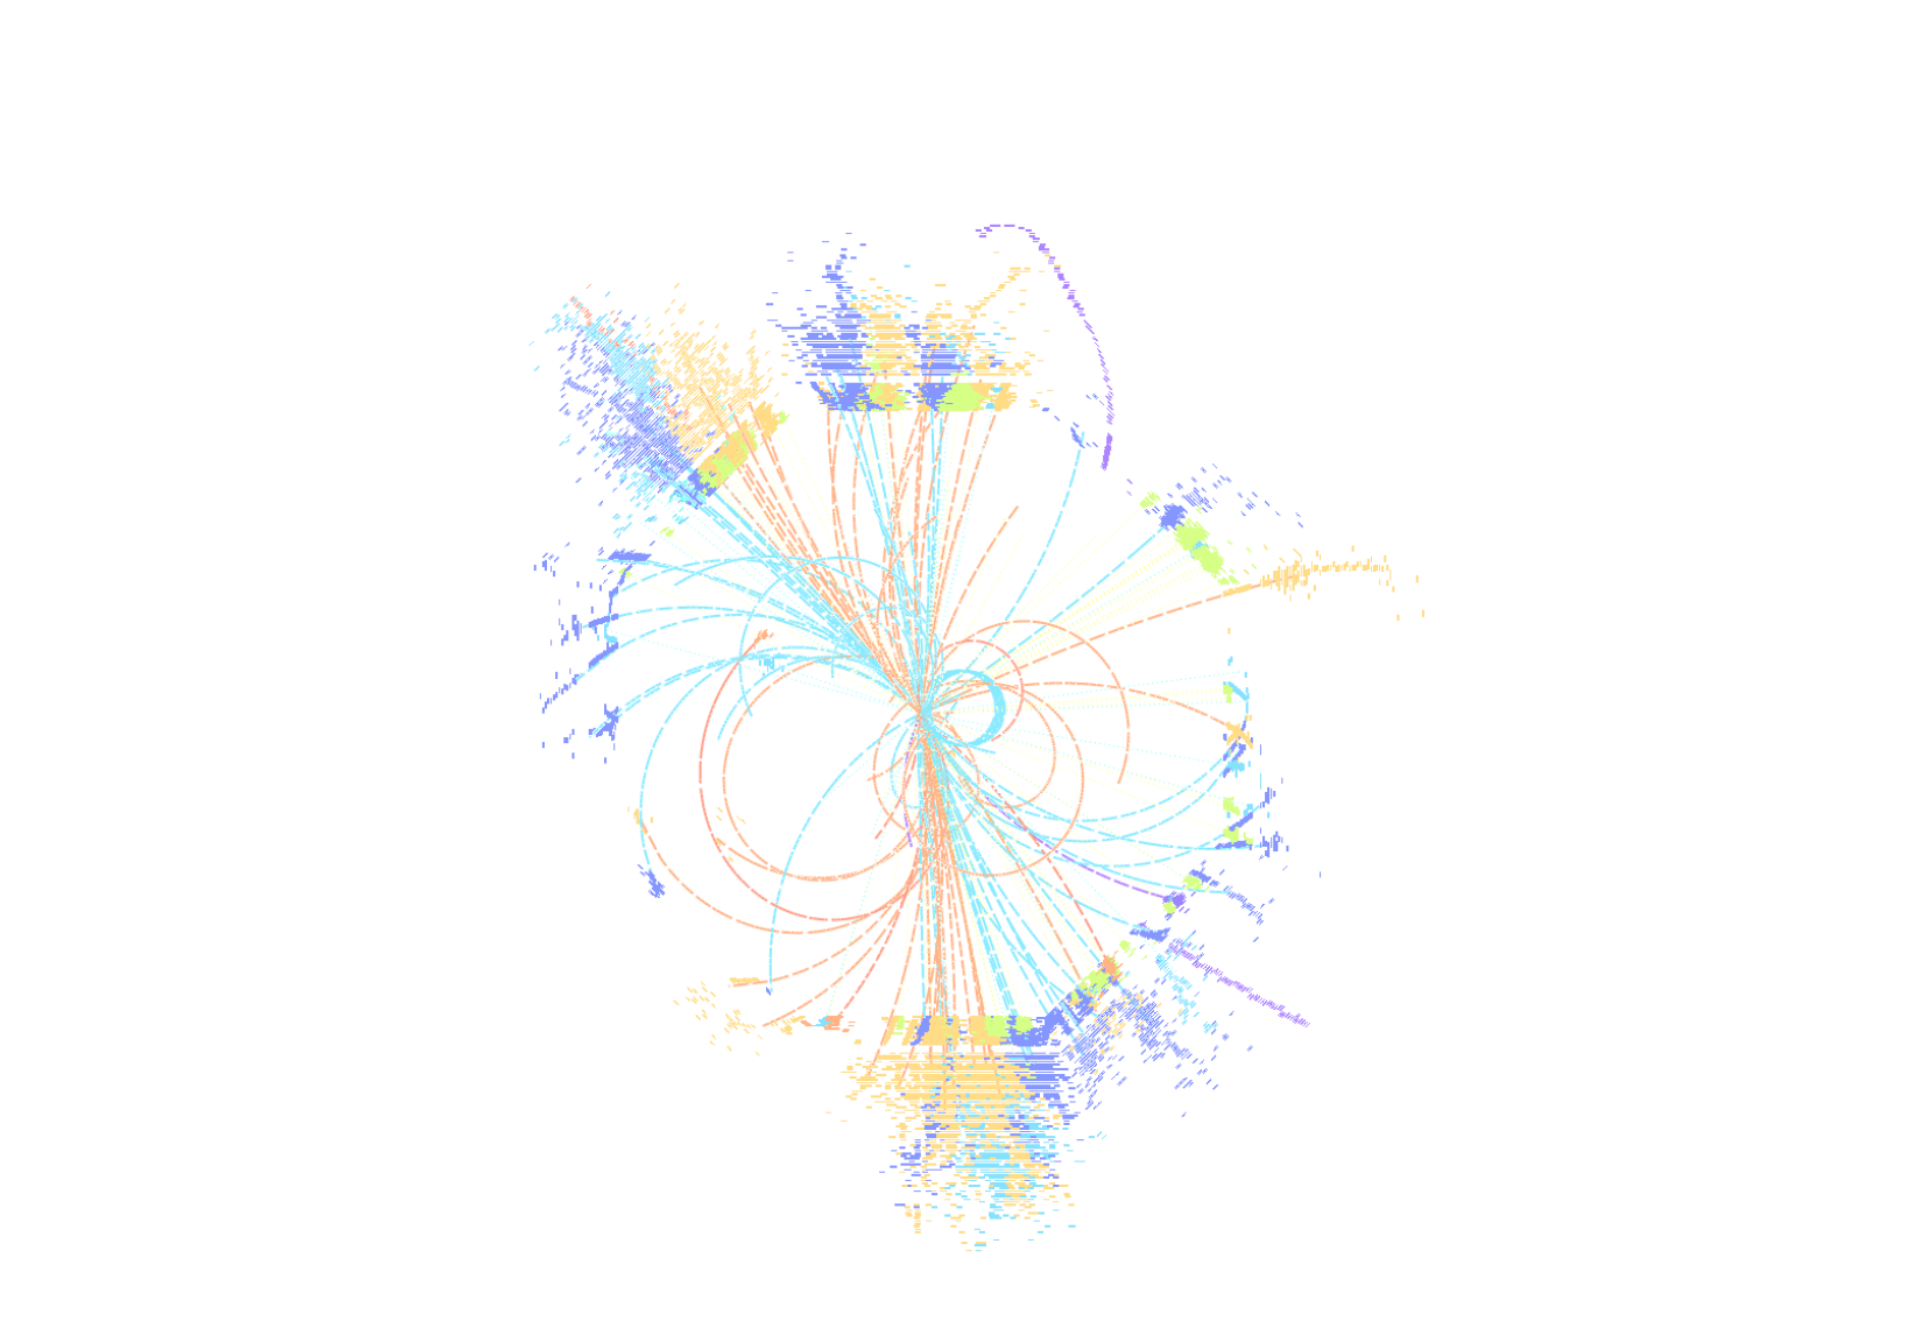
\includegraphics[width=\paperwidth]{background.png}}
	\begin{frame}<beamer>
		\frametitle{Outline}
		\tableofcontents[currentsection,currentsubsection]
	\end{frame}
}
}
\title[]{CLIC Physics and detectors CDR}
%%\subtitle{Our experience}

\date{\today}

\begin{document}

{
\usebackgroundtemplate{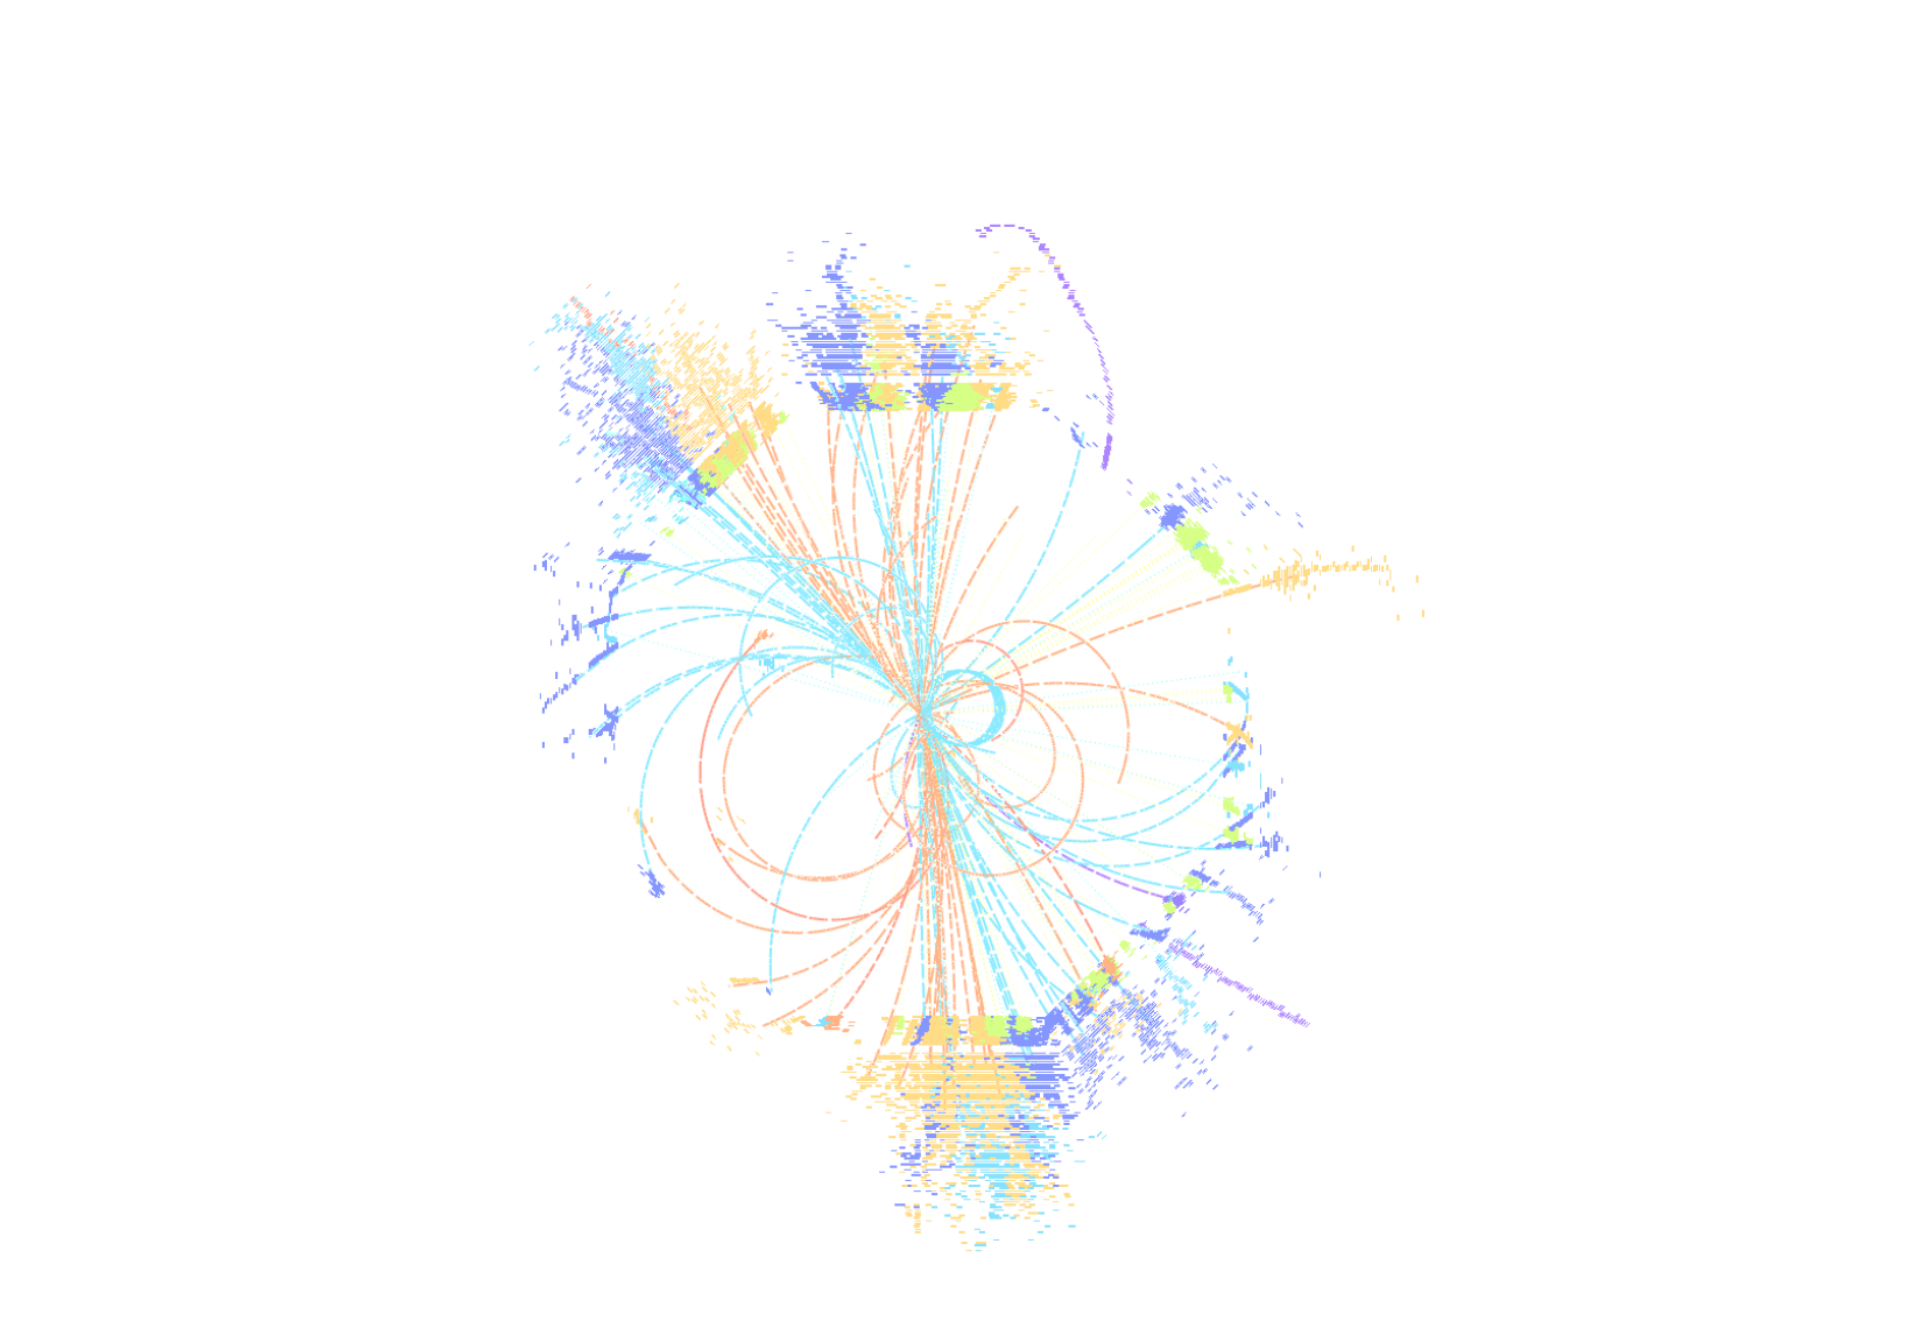
\includegraphics[width=\paperwidth]{background.png}}

\begin{frame}
	\titlepage
\end{frame}

\begin{frame}
\frametitle{Outline}
\tableofcontents
% You might wish to add the option [pausesections]
\end{frame}
}

\section[Motivations for CLIC]{Motivations for a CLIC machine}%1slide
\begin{frame}
 \frametitle{Motivations for a CLIC machine}
 CLIC: Compact LInear Collider
 \begin{itemize}
   \item $\Pep\Pem$ collisions up to $\sqrt{s}=3$TeV c.m.
   \item Machine environment challenging
\end{itemize}
~\\
CLIC physics potential:
\begin{itemize}
   \item Complementary to LHC
   \item Cleaner environment
   \item Precision Higgs physics, SUSY studies, etc.
   \item New physics beyond the LHC reach
 \end{itemize}
 
\end{frame}

\section{Physics Potential}
\begin{frame}
\frametitle{SM Higgs}
High precision measurement of its fundamental properties: mass,
total decay width, spin-parity quantum numbers, couplings to fermions and gauge bosons and
self couplings\\
\begin{columns}[c]
\column{6cm}
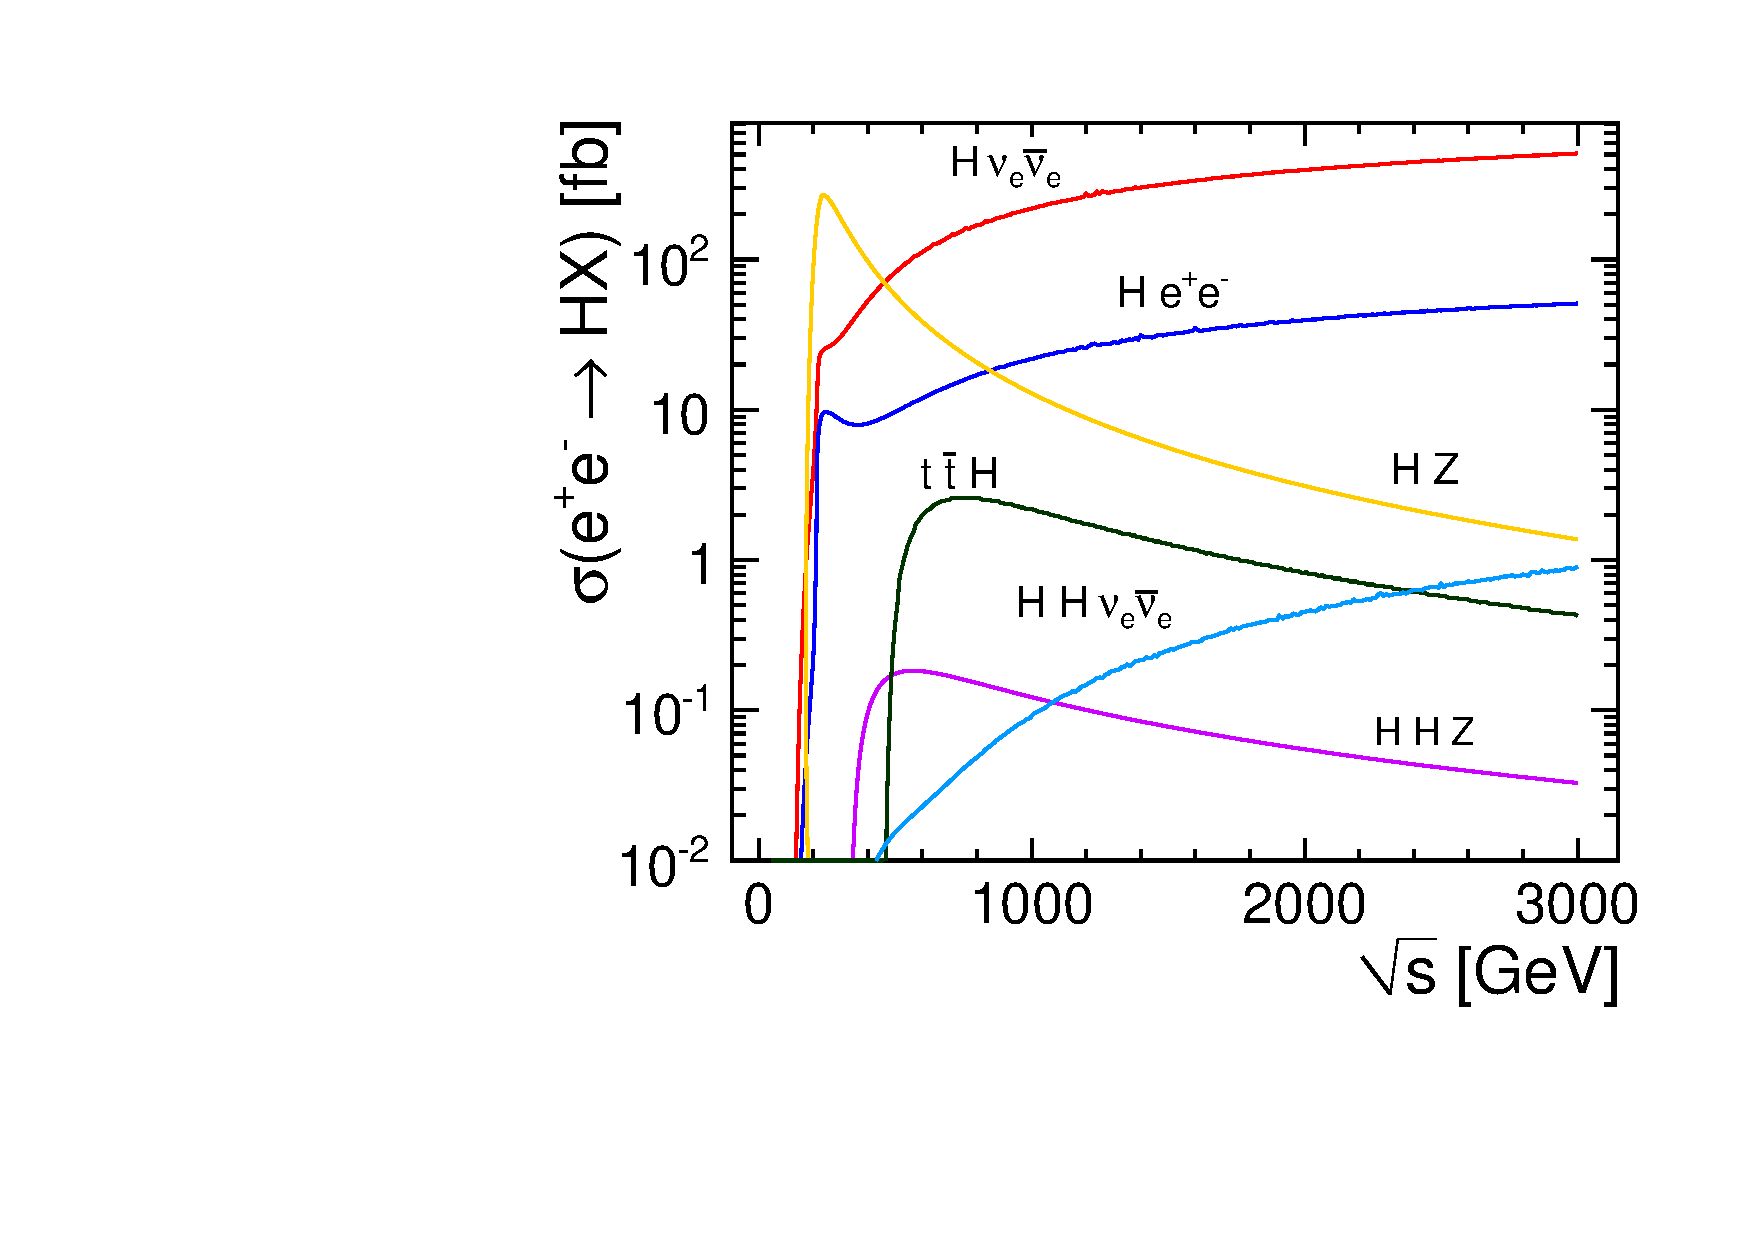
\includegraphics[width=6cm]{../SIDWorkshop/xsec_vs_cme.pdf}
\column{6cm}
\begin{center}
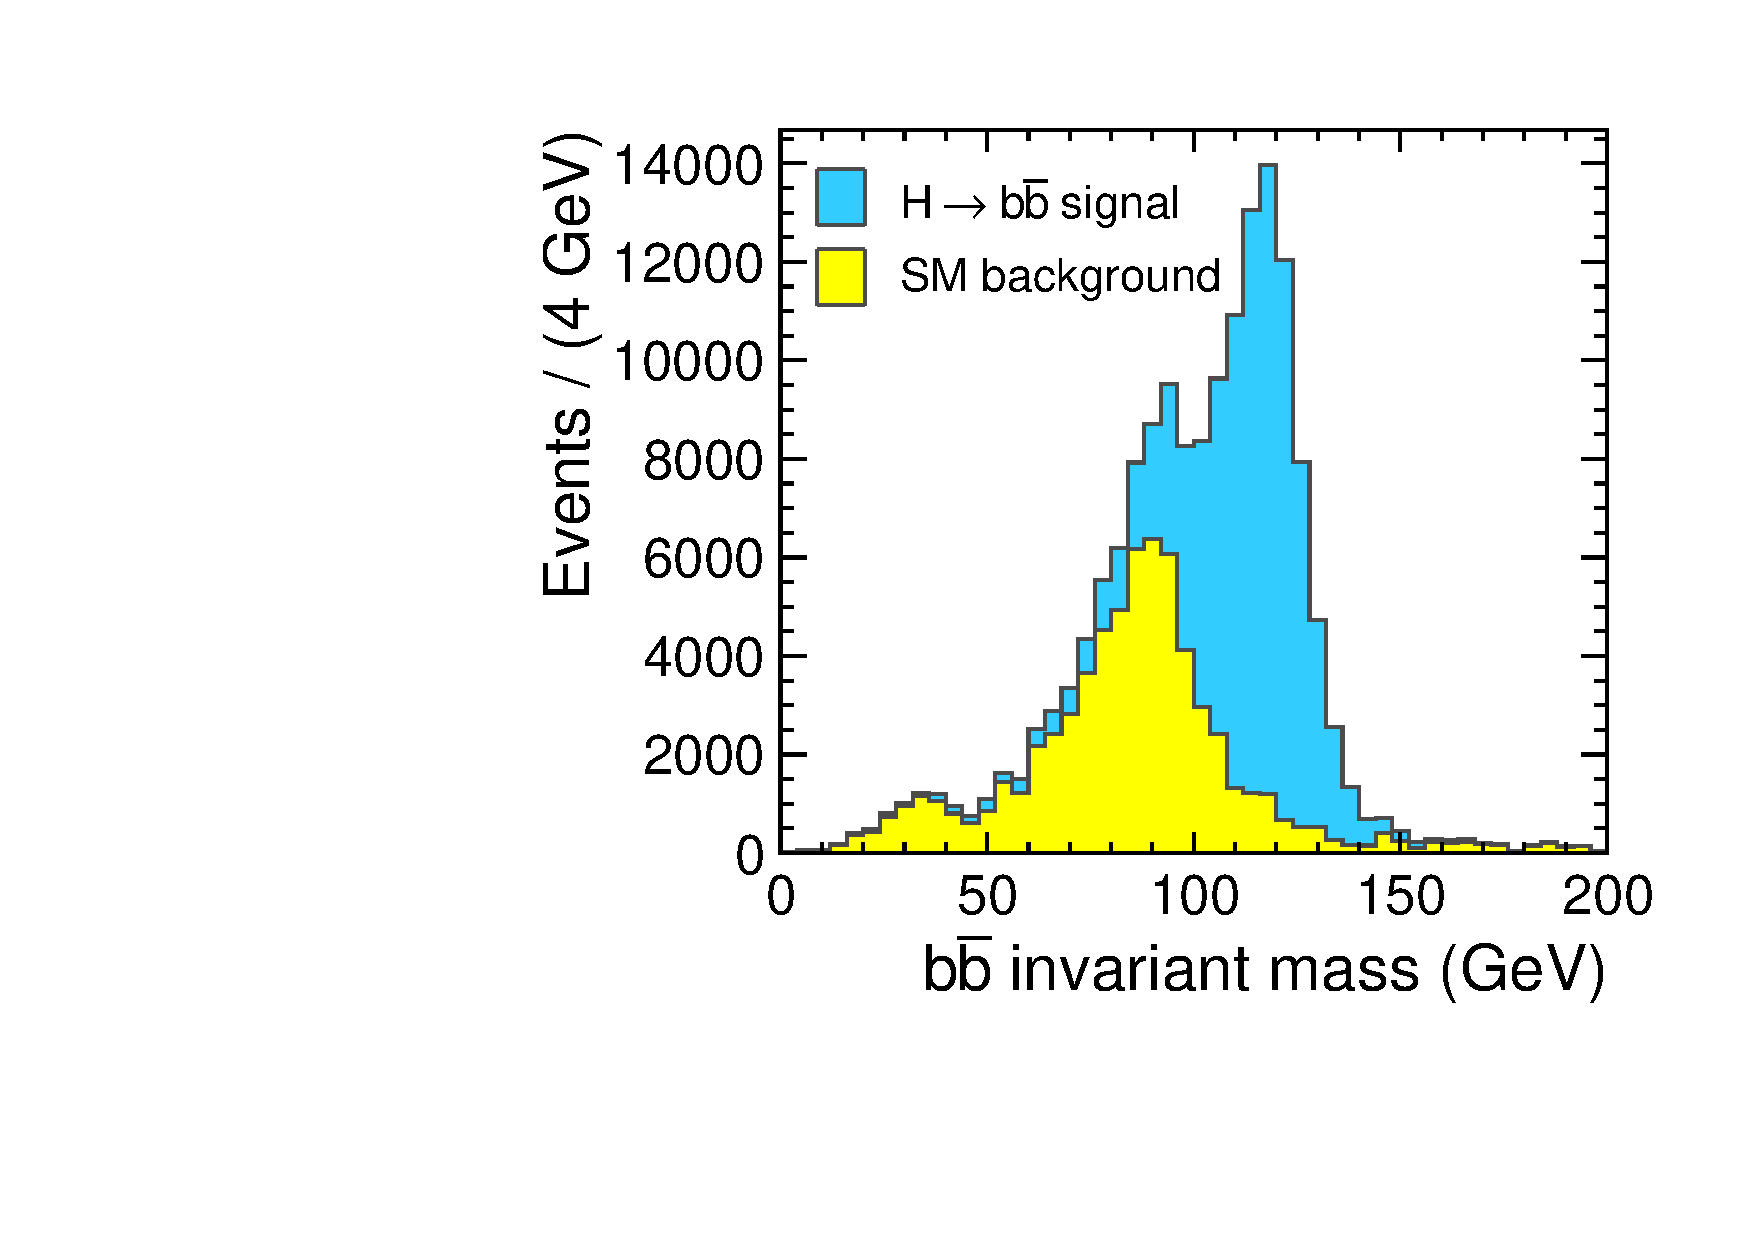
\includegraphics[width=3cm]{../SIDWorkshop/ee_h_bb_mass_mh120GeV.pdf}
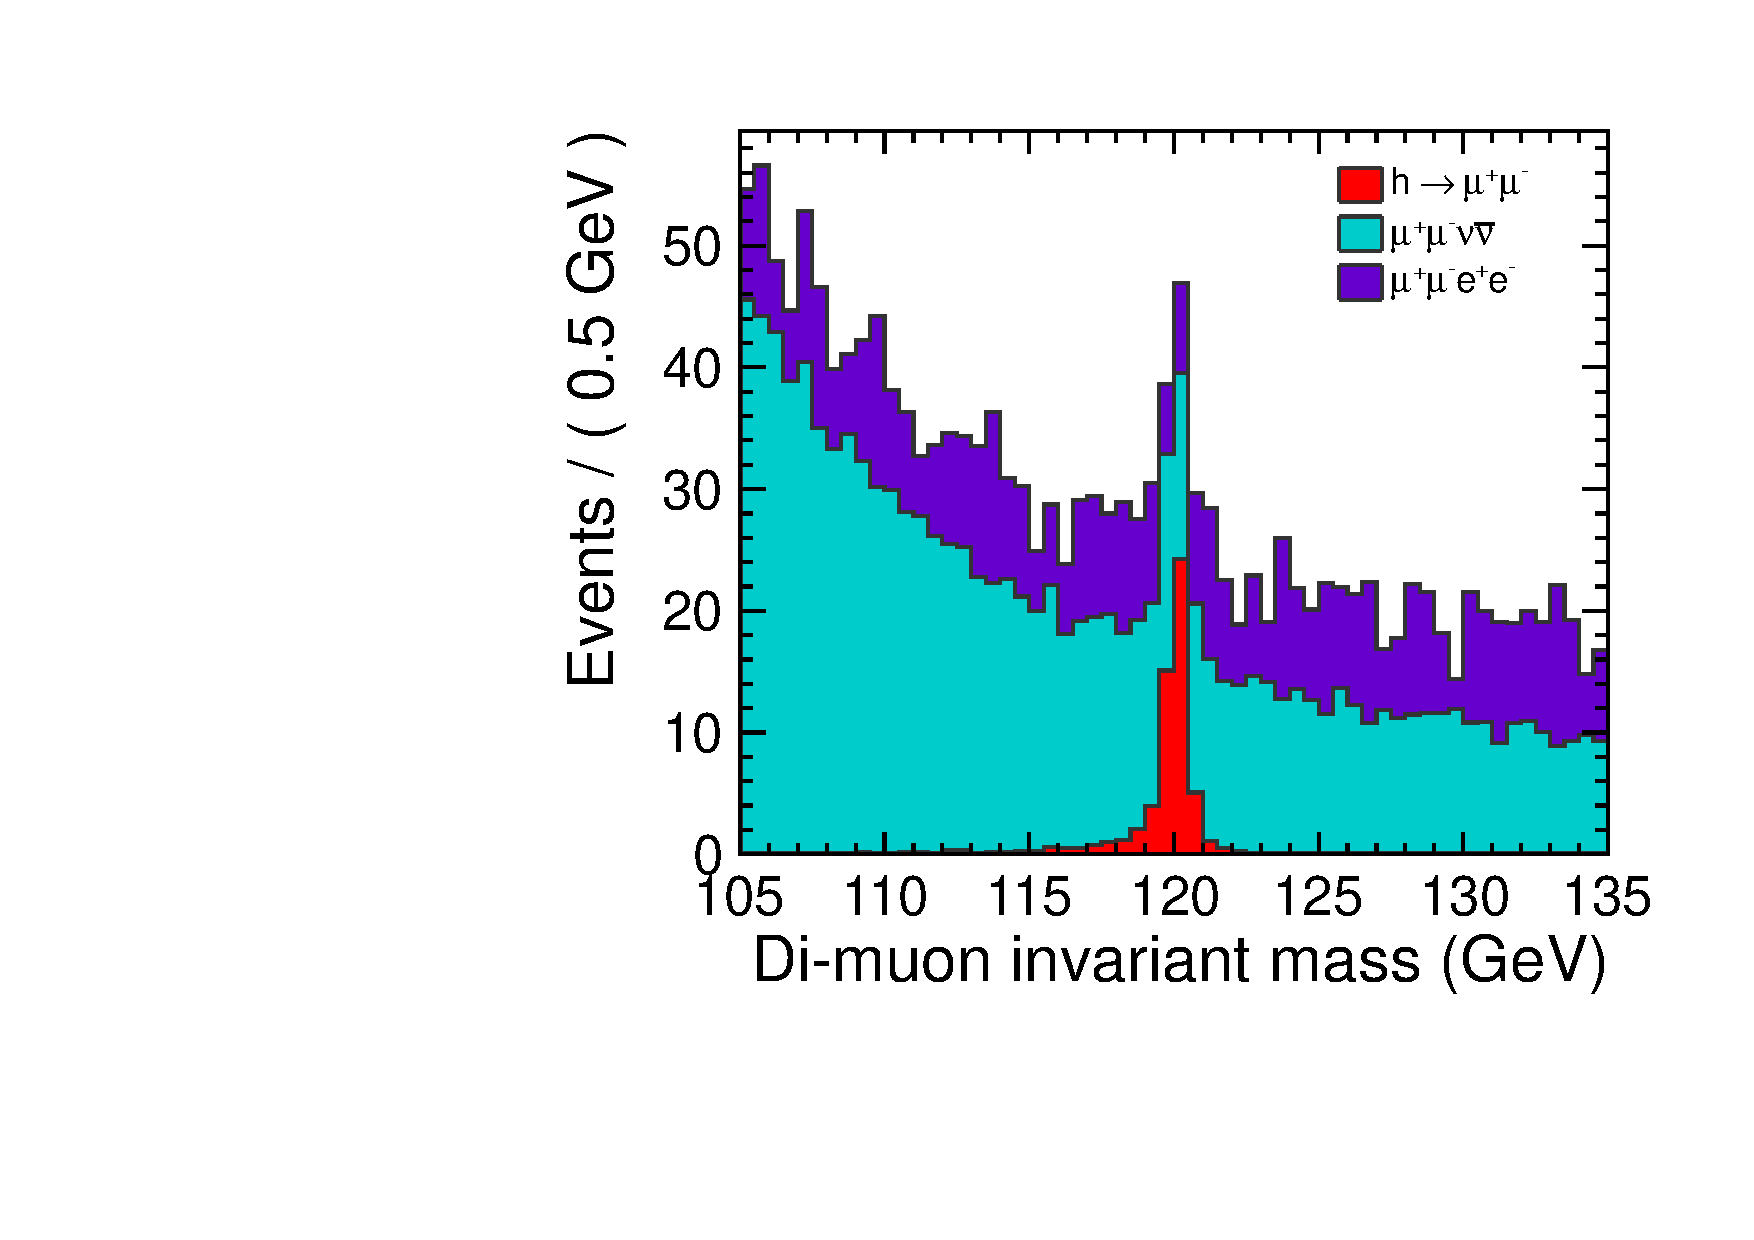
\includegraphics[width=3cm]{../SIDWorkshop/ee_h_mumu_mass_mh120GeV.pdf}\\
\begin{tabular}{cc}
Coupling & Stat. precision\\
\midrule
$g_{\PH\to\Pbottom\APbottom}$ & 2\%\\
$g_{\PH\to\Pcharm\APcharm}$ & 3\% \\
$g_{\PH\to\mu\mu}$ & 15\%\\
\bottomrule
\end{tabular}
\end{center}
\begin{tikzpicture}[remember picture, overlay, transform shape, rotate=45,]
\node<2>[inner sep=0pt, scale=1.5] at (4.5,0.) {% 
      {\Huge \alert{More later !}}%
    };%
\end{tikzpicture}
\end{columns}
Ongoing studies for self coupling $\lambda_{HHH}$.
\end{frame}

\begin{frame}
\frametitle{BSM Higgs}
\begin{columns}[c]
\column{6cm}
$\Pep\Pem \to \PH\PA \to \Pbottom\APbottom\Pbottom\APbottom$\\
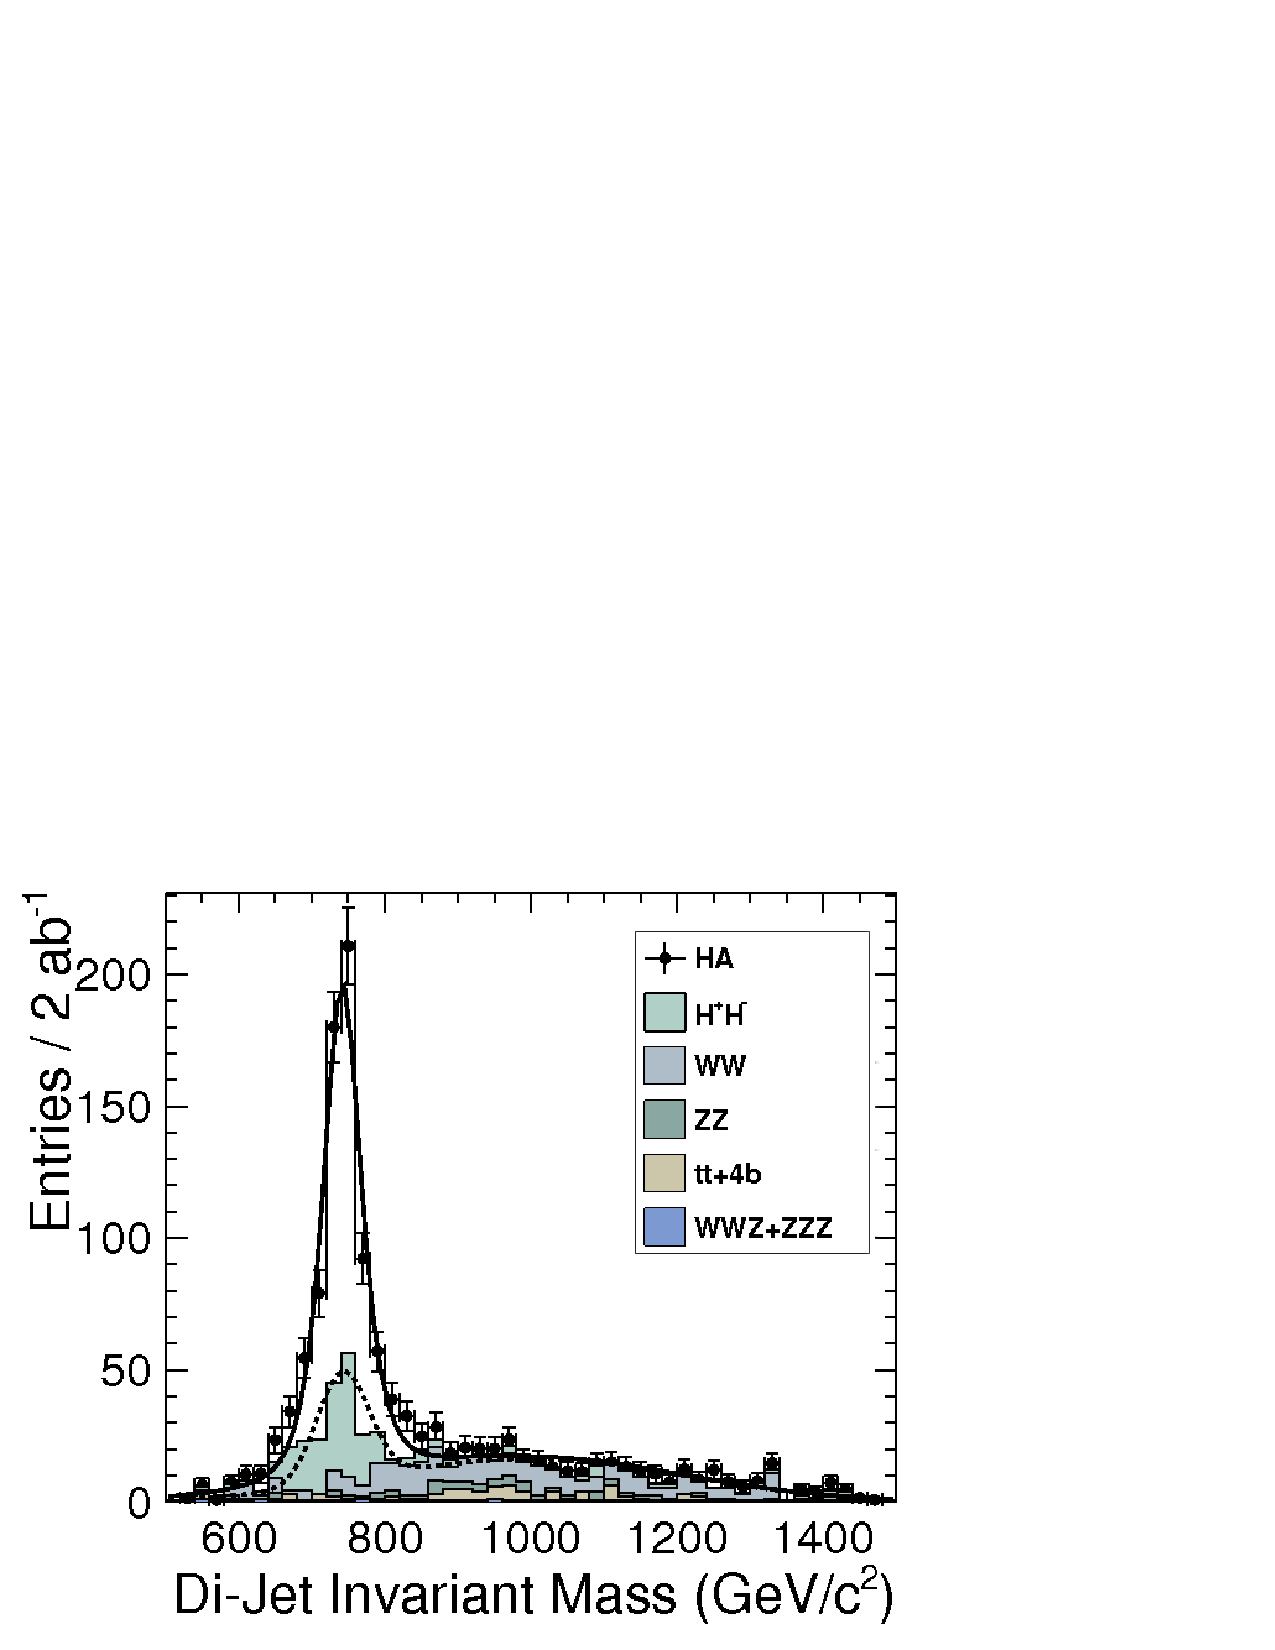
\includegraphics[width=5cm]{HAMass742_Bkg_CKFM_00BX_FJ.pdf}
\column{6cm}
$\Pep\Pem \to \PHp\PHm \to \Ptop\APbottom\APtop\Pbottom$
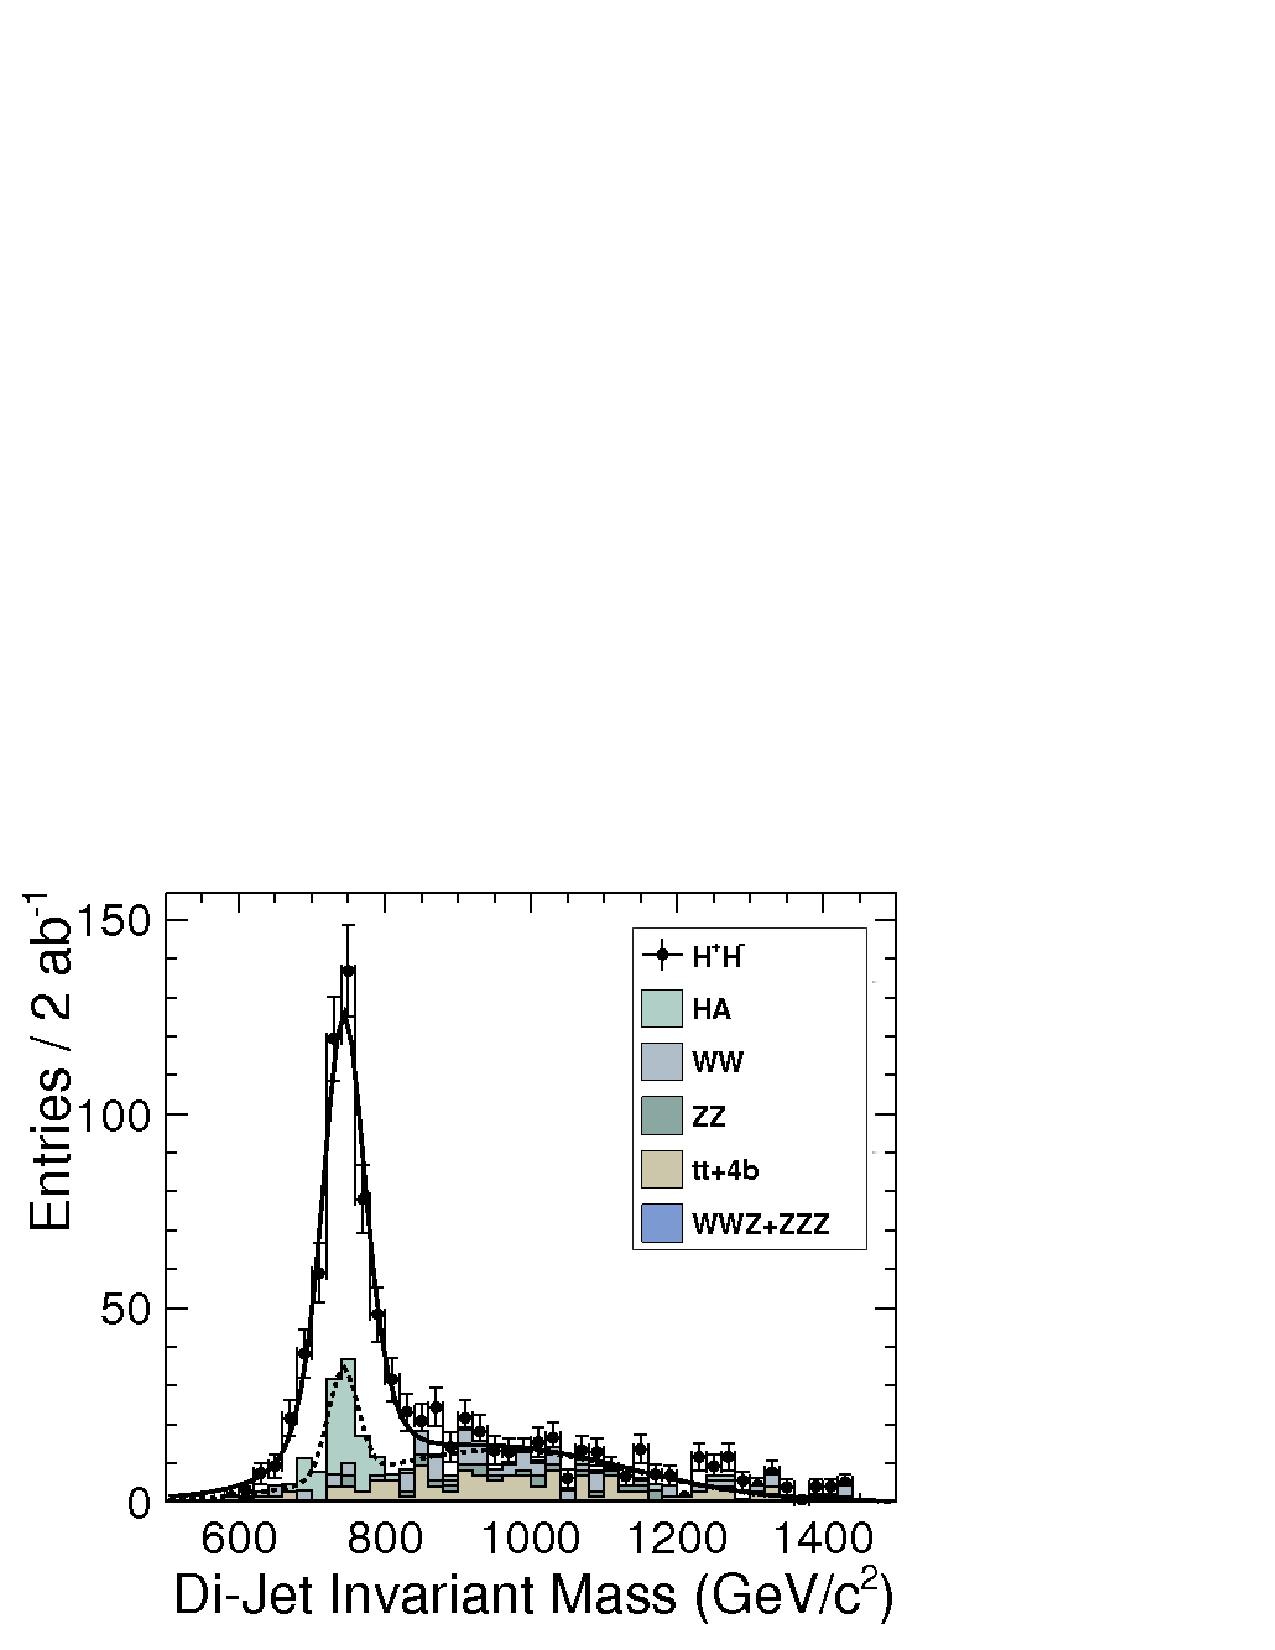
\includegraphics[width=5cm]{Hpm_Mass742_Bkg_CKFM_00BX_FJ.pdf}
\end{columns}
\begin{center}
\begin{tabular}{ccc}
\toprule
~ & $\sigma(m)/m$ & $\sigma(\Gamma)/\Gamma$\\
\midrule
$\PA/\PH$ & 0.002 & 0.10\\
$\PHpm$ & 0.005 & 0.15\\
\bottomrule
\end{tabular}
\end{center}
$\Rightarrow$ determination of $\sigma(\tan \beta)/\tan \beta <$ 0.06.
\begin{tikzpicture}[remember picture, overlay, transform shape, rotate=45,
scale=2] \node<2>[inner sep=0pt] at (current page.center) {%
        {\Huge \alert{More later !}}%
    };%
\end{tikzpicture}
\end{frame}

\begin{frame}
\frametitle{SUSY}
\begin{center}
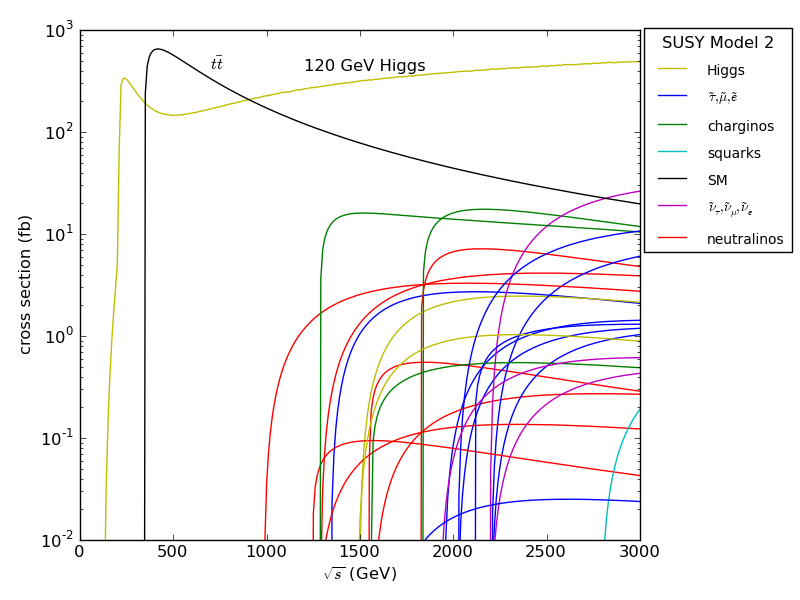
\includegraphics[width=9cm]{../SIDWorkshop/susy_model2.png}
\end{center}
Study chargino and neutralino masses by measuring kinematic endpoints of the
energy distributions, in channels like $\PSgxzii \to \Ph \PSgxzi$
\begin{tikzpicture}[remember picture, overlay, transform shape, rotate=45,
scale=2] \node<2>[inner sep=0pt] at (current page.center) {%
        {\Huge \alert{More later !}}%
    };%
\end{tikzpicture}

\end{frame}
\begin{frame}
\frametitle{SUSY}
Susy breaking models separation capability:
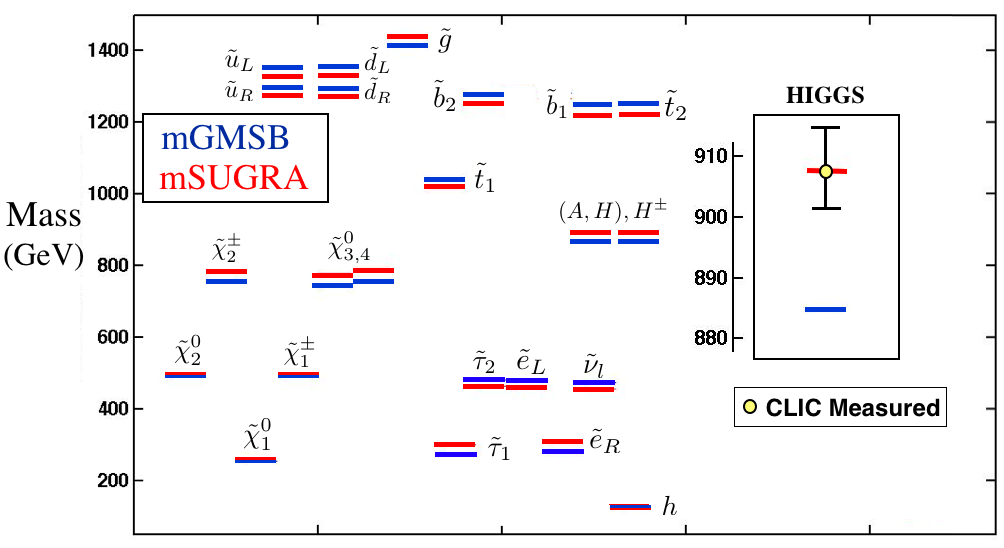
\includegraphics[width=10cm]{../SIDWorkshop/GvM.png}
\end{frame}
\begin{frame}
\frametitle{Other studies}
\begin{itemize}
  \item High scale stucture of SUSY
  \item Neutralino Dark Matter hypothesis
  \item Higgs strong interaction
  \item Z'
  \item Contact interaction
  \item Extra dimensions
\end{itemize}
\end{frame}
\begin{frame}
\frametitle{Physics potential summary}
\begin{center}
{\scriptsize
 \begin{tabular}{ ccccc }
    \toprule
 Machine &     LHC14 & SLHC & LC800 & CLIC3\\
 Luminosity & $100\textrm{fb}^{-1}$ & $1\textrm{ab}^{-1}$&
 $500\textrm{fb}^{-1}$& $1\textrm{ab}^{-1}$\\
\midrule
squarks [TeV] &   2.5 & 3 & 0.4 & 1.5 \\
sleptons [TeV] &   0.3 & - & 0.4 & 1.5 \\ 
$\textrm{Z}'$ ({\tiny SM ~couplings}) [TeV]  &  5 & 7 & 8 & 20   \\ 
%\Zprime ({\tiny SM~couplings})  &     5& 6  & 8 & 22 \\
%$q*$      &    6.5 & 7.5 & 0.8 & 3 \\
%$l*$       &   3.4 & - & 0.8 & 3 \\
2 extra dims $M_D$ [TeV]  &    9 & 12 & 5-8.5 & 20-30 \\
%$W_L W_L$      &  3.4sig& >3.4sig& -& 70sig\\
TGC (95\%)  ({\tiny \rm $\lambda_{\gamma} $~coupling}) &   0.001& 0.0006& 0.0004& 0.0001 \\
$\mu$ contact scale [TeV] &  15& - & 20 & 60 \\
Higgs compos. scale [TeV] & 5-7 & 9-12 & 45 & 60\\
    \bottomrule
  \end{tabular}
  }
 \end{center}
 CLIC can 
 \begin{itemize}
   \item extend the \alert{discovery reach} of LHC,
   \item offer the opportunity of \alert{precise measurements} of masses and
 couplings.
 \end{itemize}
\end{frame}


\section[CLIC]{The CLIC Machine}
\begin{frame}
\frametitle{CLIC machine Conceptual Design Report}
\begin{itemize}
  \item Released later in 2012
  \item Presents the different technical aspects of a CLIC machine
  \item Details the machine properties
\end{itemize}
Here: brief overview of those properties
\end{frame}
\begin{frame}
\frametitle{CLIC Technology}
\begin{columns}[c]
\column{6cm}
2 beam acceleration scheme: drive beam and main beam
\begin{itemize}
  \item Gradient 100 MV/m
  \item Energy: from few-hundred GeV upgradable in steps up to 3 TeV; R\&D has
  focused on 3 TeV
\end{itemize}
\column{6cm}
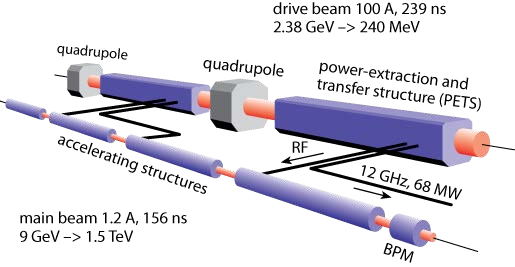
\includegraphics[width=6cm]{clicacceleration.png}
\end{columns}
\end{frame}

\begin{frame}
\frametitle{CLIC properties}
compare to LHC/ILC
\begin{center}
\begin{tabular}{ccc}
 & ILC 0.5TeV & CLIC 3TeV\\
 \midrule
L [$\textrm{cm}^{-2}\,\textrm{s}^{-1}$] & $2\times 10^{34}$&$5.9\times 10^{34}$ \\
\midrule
Bunch crossing separation  & 700 ns & \alert{0.5 ns}\\
\midrule
Bunch crossings per train & 2670 & \alert{312}\\
\midrule
Train repetition rate  & 5 Hz & 50 Hz\\
\midrule
Crossing angle & 14mrad & 20mrad\\
\bottomrule
\end{tabular}
\end{center}
\alert{Whole bunch train in 156ns.}
\end{frame}
\begin{frame}
\frametitle{Machine Detector Interface}
Push-Pull system:\\
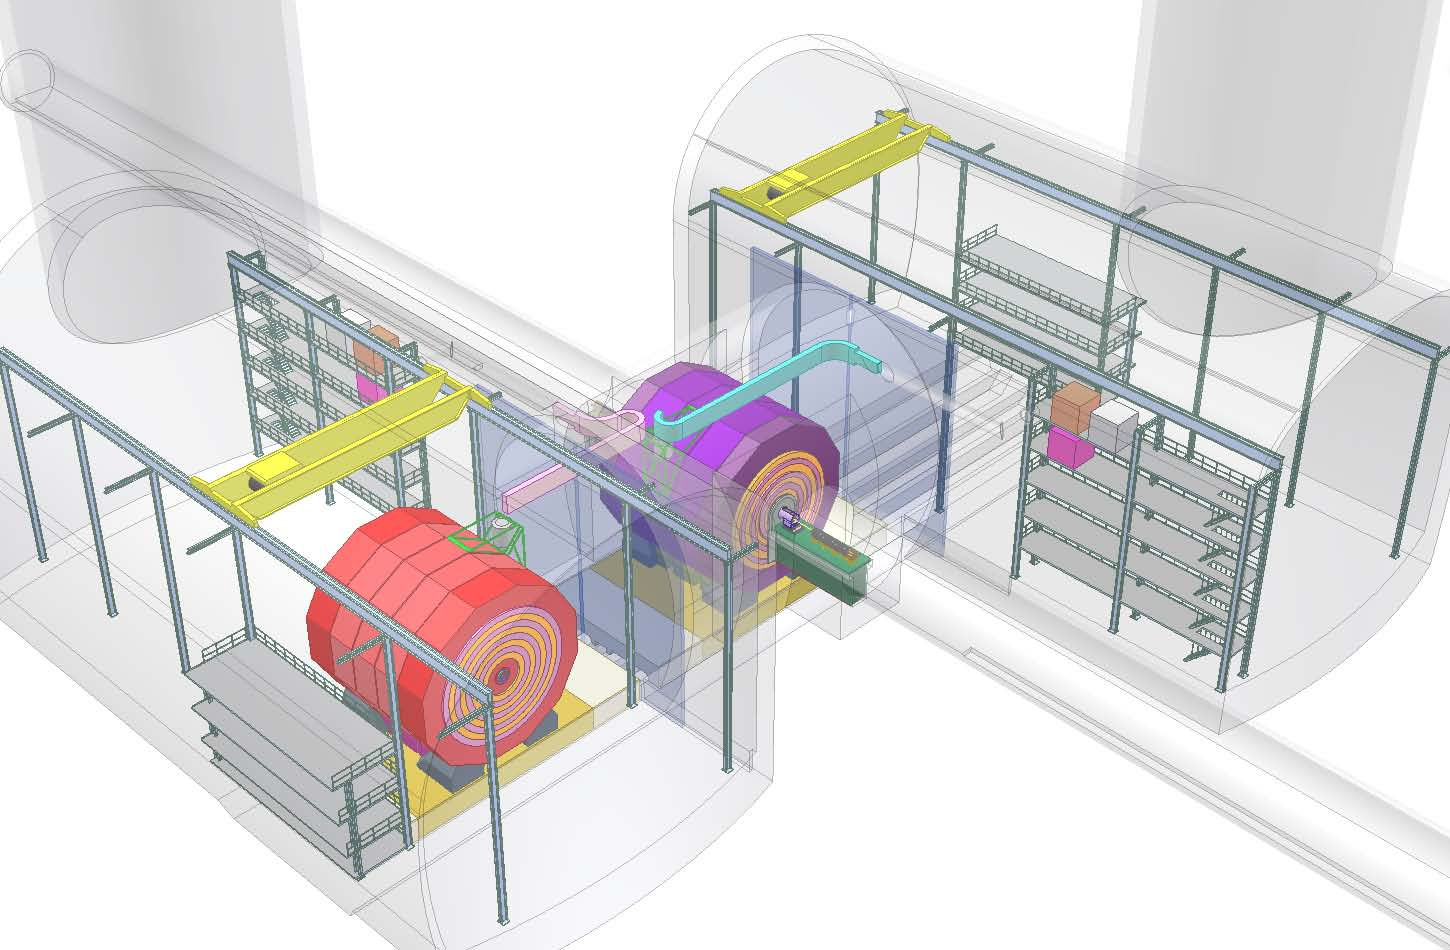
\includegraphics[width=10cm]{PushPull.png}
\end{frame}
\begin{frame}
\frametitle{Machine Detector Interface}
\begin{center}
\begin{tikzpicture}[scale=1] 
\node[] (0.0, -0.3) {\includegraphics[width=10cm,clip,trim= 0 0 0
0]{Figure_13_14.pdf}}; 
\draw<1>[<-,ultra thick, red] (-1.0,0.0)  to[] (-1.0,-3.5);
\end{tikzpicture}
\alert{Last accelerator element is IN the detector}
\end{center}
\end{frame}

\begin{frame}
\frametitle{Machine induced backgrounds}
\begin{tabular}{ccc}
 & ILC 0.5TeV & CLIC 3TeV\\
\hline
Nb $\gamma\gamma\to\textrm{had}$/BX & 0.2 & \alert{3.2}\\
\hline
Nb incoherant pairs/BX & $1\times 10^5$ & \alert{$3\times10^5$}\\
\hline
Nb coherent pairs/BX & $<10^2$ & $7\times 10^8$\\
\hline
\end{tabular}\\
~\\
\alert{Very large machine induced background rates!}\\
\begin{itemize}
  \item Coherent pairs very forward
  \item Incoherent pairs mostly forward
\end{itemize}
$\to$ impact on the very forward detectors design\\
~\\
\begin{itemize}
  \item $\gamma\gamma\to\textrm{hadrons}$ all over the detector acceptance.
\end{itemize}
\alert{Need to deal with those}
\end{frame}

\section[Detectors]{The Detectors}
\begin{frame}
\frametitle{Required performance}
\begin{itemize}
  \item Trigger less readout of full train: time stamping, multi-hit capacity,
  filtering algorithms during reconstruction
  \item High resolution pixel detector for displaced vertices identification:\\
  {\scriptsize
  \begin{tabular}{lc}
  p = 1 Gev & $\sigma_{d0}\sim20\mu m$\\
  p = 100 GeV & $\sigma_{d0}\sim5\mu m$
  \end{tabular}
  }~\\ ~\\
  \item Momentum resolution:\\
  {\scriptsize 
  $\sigma(p_{\textrm{T}})/p_{\textrm{T}}^2\sim 10^{-5}\textrm{GeV}^{-1}$
   }~\\ ~\\
  \item Good jet-energy resolution (W/Z separation)\\
  {\scriptsize 
$\sigma(E_j)/E_j = 3.5\%-5\%$ for $E_j = 50\textrm{GeV}-1\textrm{TeV}$
  }~\\ ~\\
\end{itemize}
\end{frame}
\begin{frame}
\frametitle{Particle Flow Paradigm}
Jet energy:
\begin{itemize}
  \item 60\% carried by charged particles
  \item 30\% by photons
  \item 10\% by long-lived neutral hadrons
\end{itemize}
Particle Flow: reconstruction of the \alert{4-momenta of all visible
particles}:
\begin{itemize}
  \item momenta measured in the tracking detectors for charged particles
  \item energy measured in the calorimeters for photons and neutral hadrons
\end{itemize}
$\Rightarrow$ need for \alert{high precision tracking and high granularity
calorimeters}
\end{frame}
\begin{frame}
\frametitle{Overview}
\begin{columns}[c]
\column{6cm}
\centering
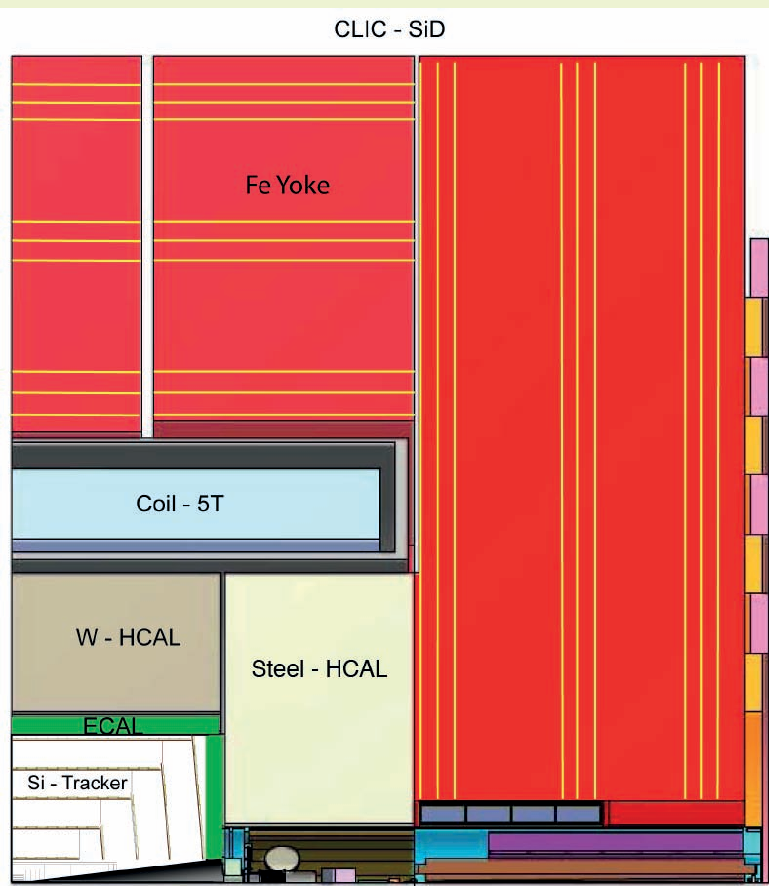
\includegraphics[width=5cm]{../SIDWorkshop/CLIC_SiD_xz.pdf}
\column{6cm}
\centering
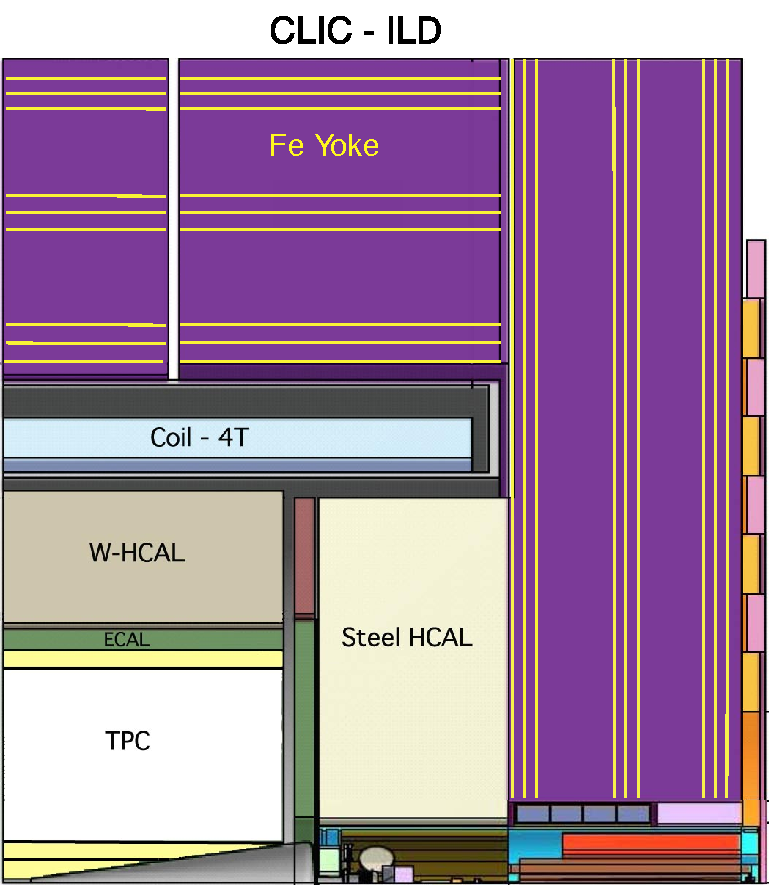
\includegraphics[width=5cm]{../SIDWorkshop/CLIC_ILD_xz.pdf}
\end{columns}
\end{frame}
\begin{frame}
\frametitle{Vertex detector optimization}
\begin{center}
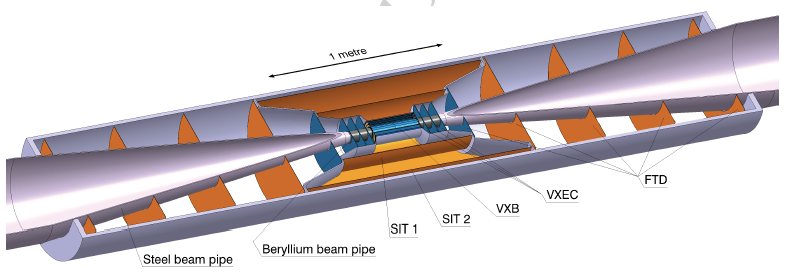
\includegraphics[width=8cm]{VertexDetector.png}
\end{center}
\begin{itemize}
  \item $20\times20\mu m$ pixel size
  \item 0.2\% X$_0$ material per layer (very thin)
  \item Time stamping 10ns
  \item Triggerless readout
  \item Radiation level $<10^{11} n_{eq}cm^{-2}year^{-1}  \Leftarrow 10^4
  \times$ lower than LHC
\end{itemize}
\alert{Challenging R\&D project}
\end{frame}

\begin{frame}
\frametitle{Tracking in CLIC\_SiD}
\begin{columns}[c]
\column{6cm}
\begin{center}
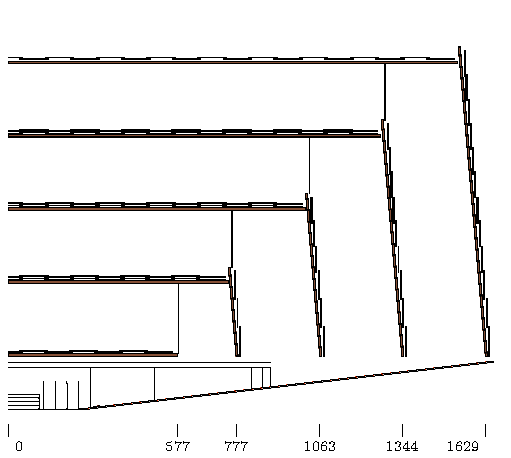
\includegraphics[width=6cm]{sid_tracker_zx.pdf}
\end{center}
\column{6cm}
\begin{itemize}
  \item All silicon tracking
  \item Efficiency ($p_{\textrm{T}}>1$GeV): $>99\%$
  \item Mom. resolution: $\sigma(\Delta(p_{\textrm{T}})/p_{\textrm{T}}^2)<
  2\cdot10^{-5}/$GeV
\end{itemize}
\alert{Compatible with requirements}
\end{columns}
\end{frame}
\begin{frame}
\frametitle{Tracking in CLIC\_ILD}
\begin{columns}[c]
\column{6cm}
\begin{center}
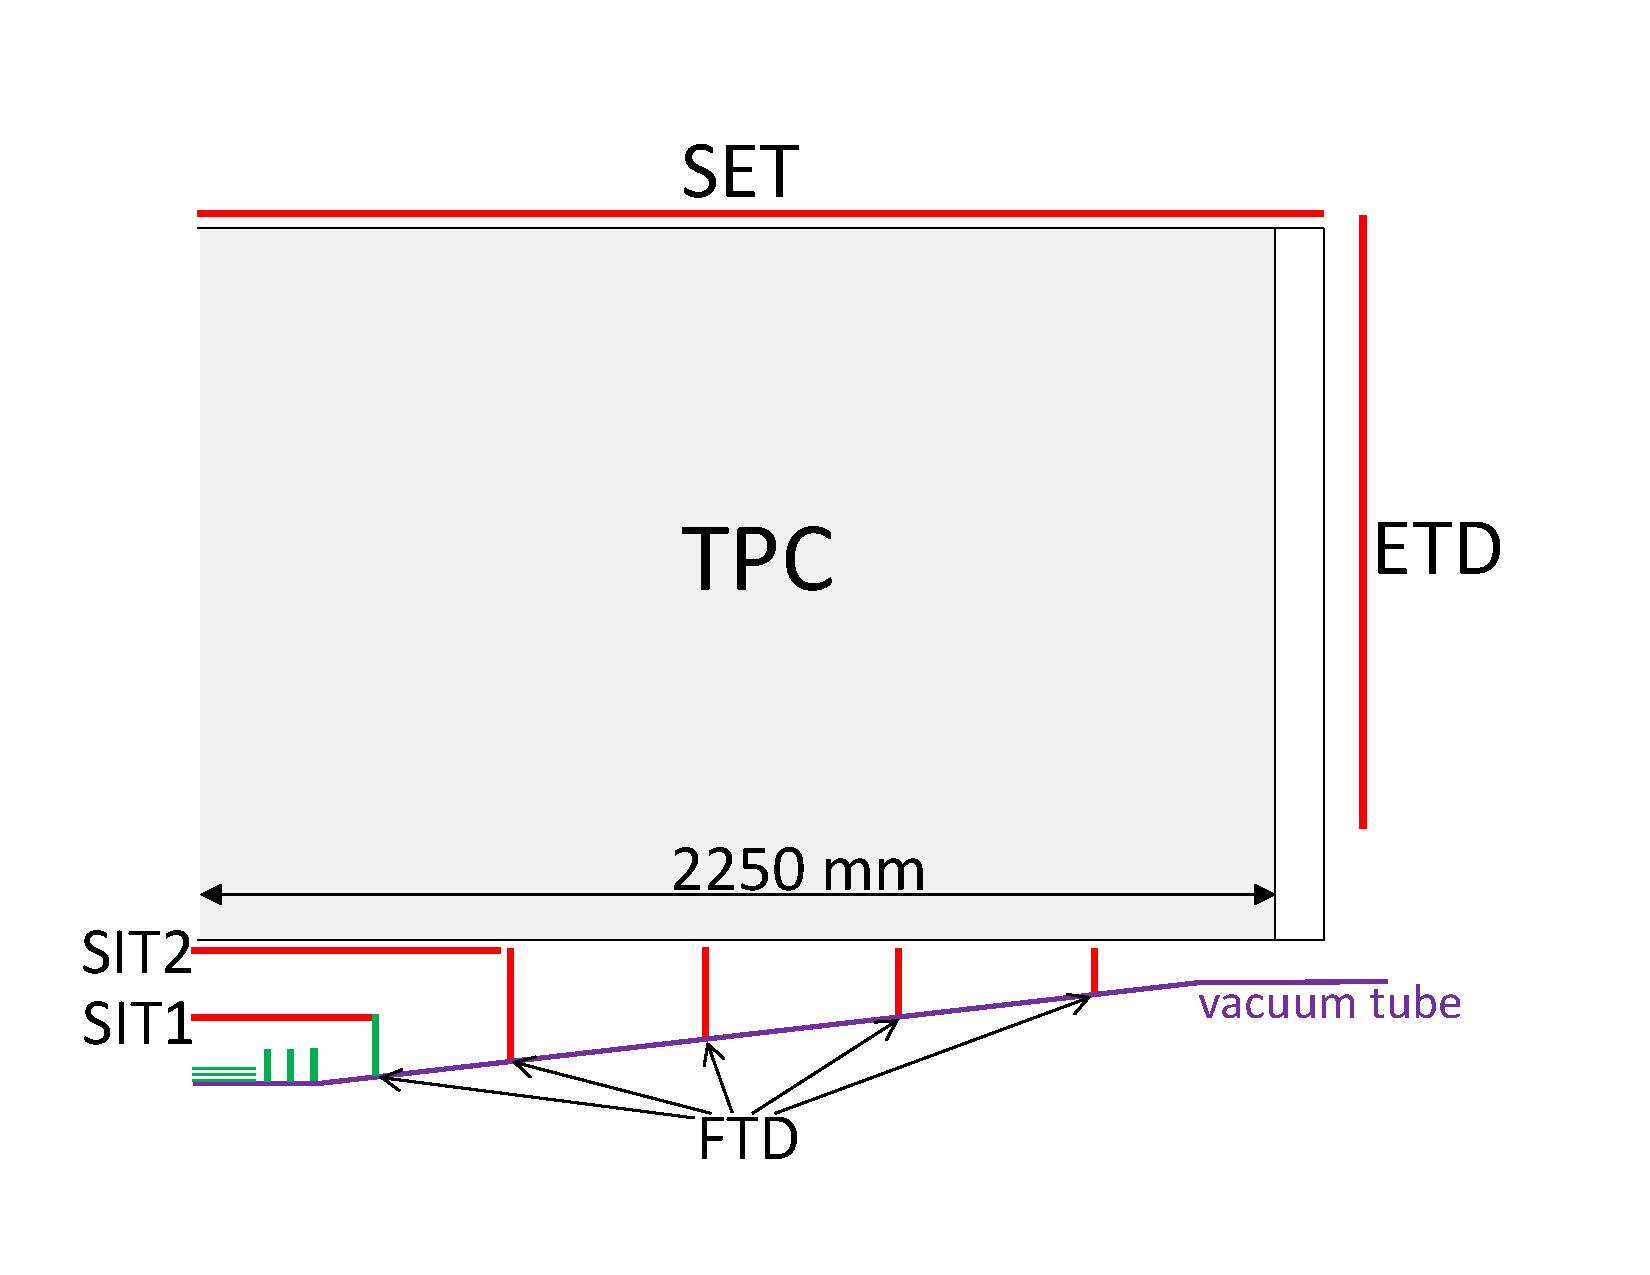
\includegraphics[width=6cm]{CLIC_ILD_tracking_geom.pdf}
\end{center}
\column{6cm}
\begin{itemize}
  \item Time Projection Chamber
  \item Completed by silicon layers
  \item Efficiency ($p_{\textrm{T}}>1$GeV): $>99\%$
  \item Mom. resolution: $\sigma(\Delta(p_{\textrm{T}})/p_{\textrm{T}}^2)\sim 2\cdot10^{-5}/$GeV
\end{itemize}
\alert{Compatible with requirements}
\end{columns}
\end{frame}
\begin{frame}
\frametitle{ECAL}
Use tungsten Fine grained for Particle Flow
\end{frame}
\begin{frame}
\frametitle{HCAL}
Use tungsten for lower depth
\end{frame}
\begin{frame}
\frametitle{CALICE results}
\end{frame}

\section[Bkg treatment]{Dealing with the machine induced background}
\begin{frame}
\frametitle{Background properties}
Main problematic background: $\gamma\gamma\to\textrm{hadrons}$
\begin{columns}[c]
\column{6cm}
\centering
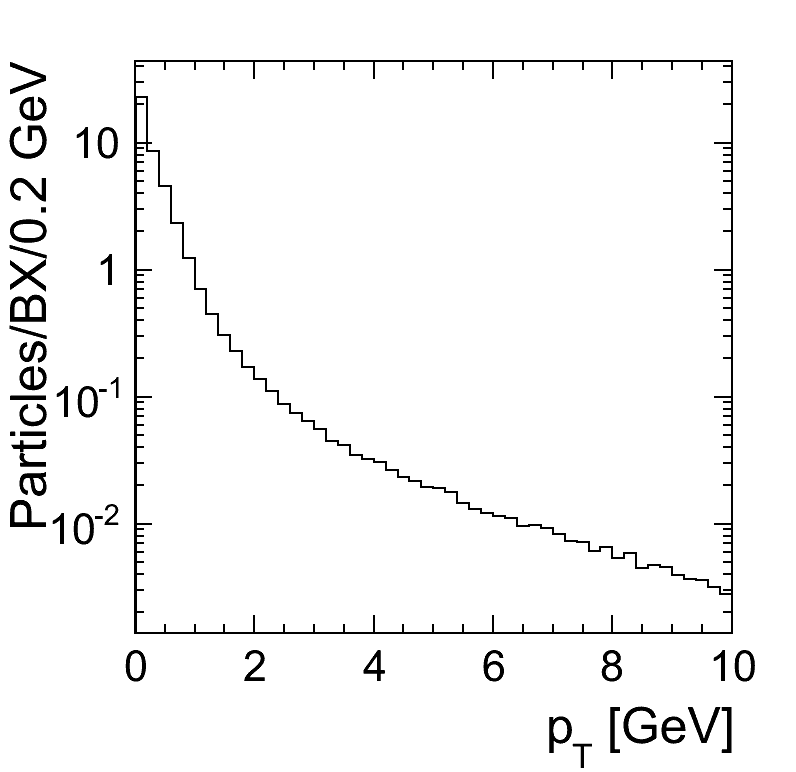
\includegraphics[width=4cm]{../SIDWorkshop/ggPT}\\
$\theta>8^\circ$
\column{6cm}
Entire bunch train (312BX):
\begin{itemize}
  \item 5000 tracks $\to$ total track momentum: \alert{7.3TeV}
  \item Total calorimetric energy (ECAL+HCAL): \alert{19TeV}
\end{itemize}
Mostly low $p_{\textrm{T}}$
\end{columns}
\end{frame}
\begin{frame}
\frametitle{Timing cuts}
\begin{columns}[c]
\column{5cm}
\centering
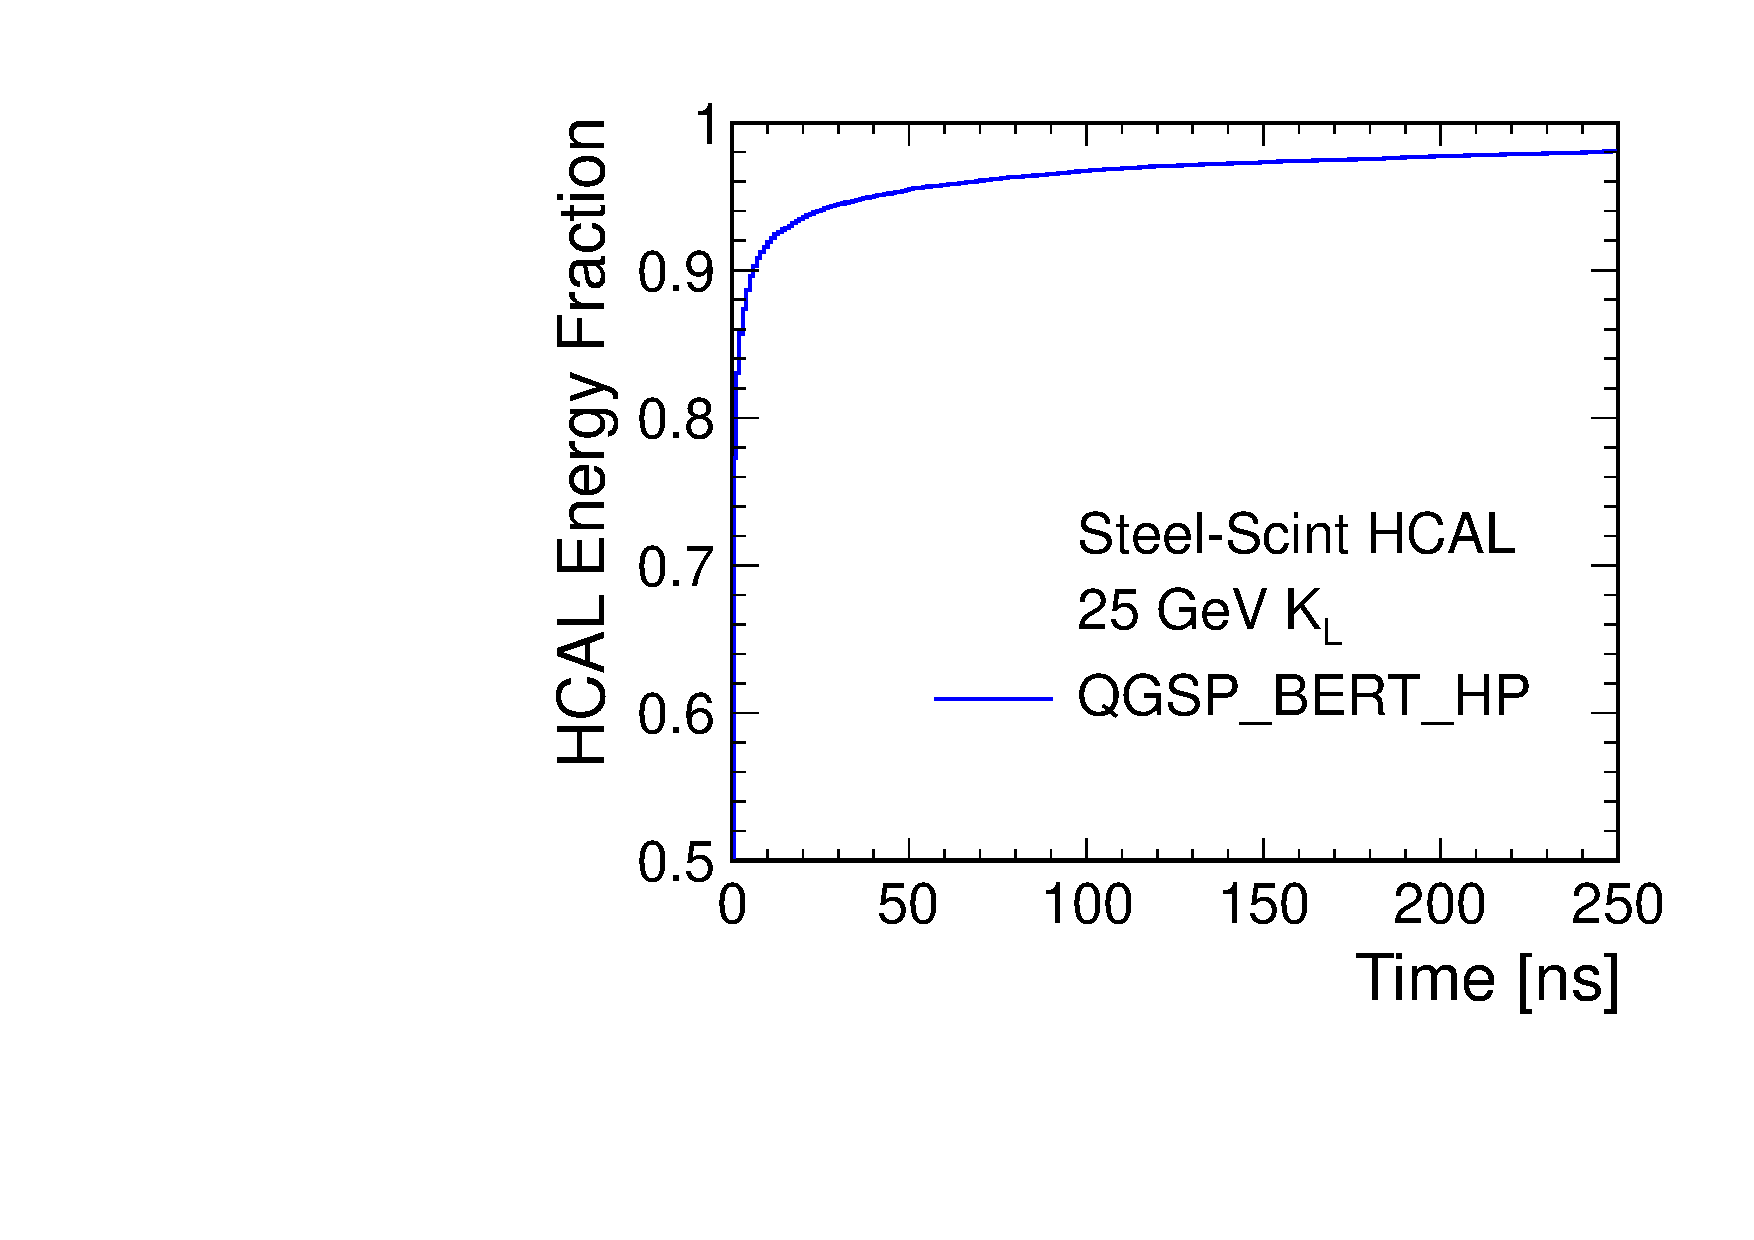
\includegraphics[width=5cm]{../SIDWorkshop/hcalTimingSteel.pdf}
\column{5cm}
\centering
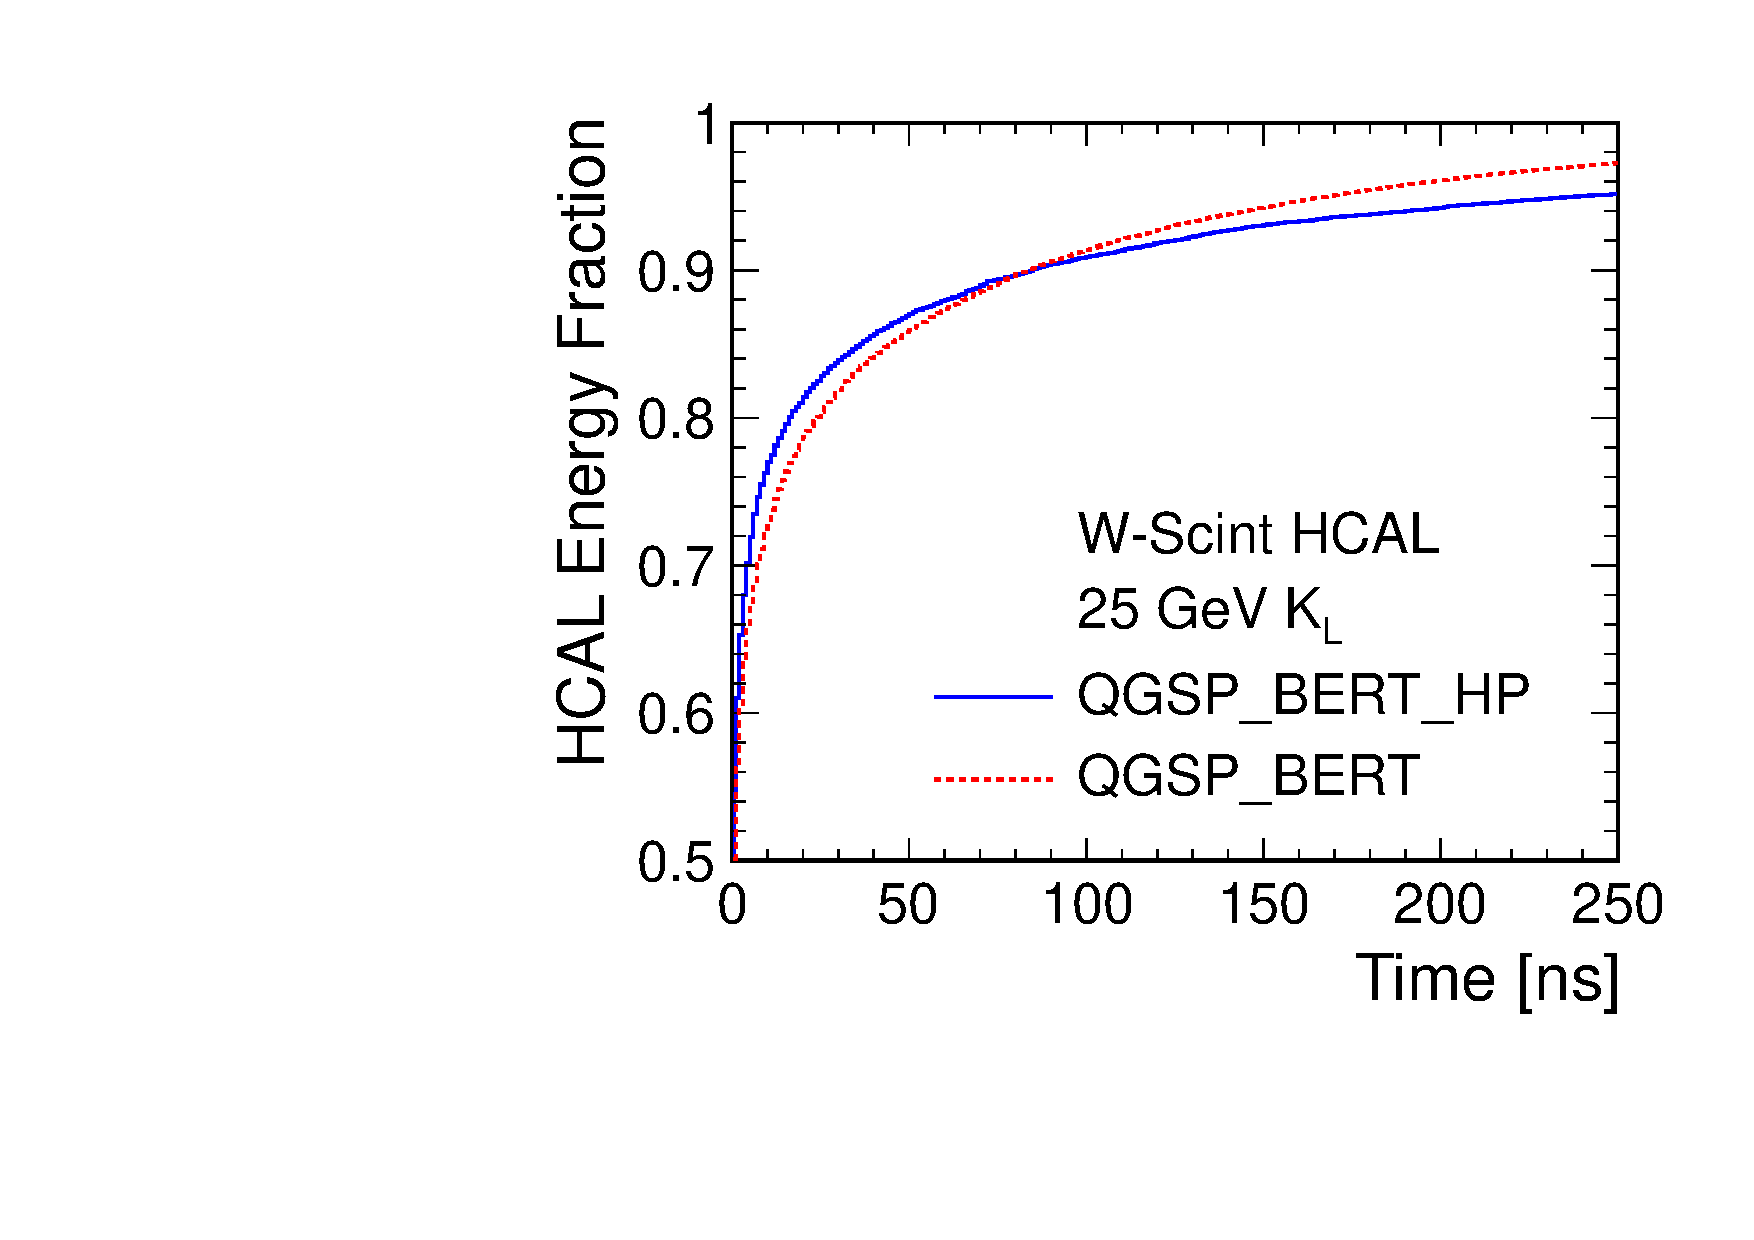
\includegraphics[width=5cm]{../SIDWorkshop/hcalTimingTungsten.pdf}
\end{columns}
\begin{center}
\begin{tabular}{lrr}
Subdetector &Reco. window &hit resolution\\
ECAL &10 ns &1 ns\\
HCAL Endcaps &10 ns &1 ns\\
HCAL Barrel &100 ns &1 ns\\
Silicon Detectors &10 ns &$10/\sqrt{12}$ ns\\
TPC & entire bunch train & n/a
\end{tabular}
\end{center}
\end{frame}
\begin{frame}
\frametitle{Jet finder}
$\Pep\Pem\to\PSq_R\PaSq_R\to\Pquark\APquark\PSgxz_1 \PSgxz_1$: 2 jets $+$
missing energy\\ ~\\
\begin{columns}[c]
\column{6cm}
Durham $k_{\textrm{T}}$ \`a la LEP:\\
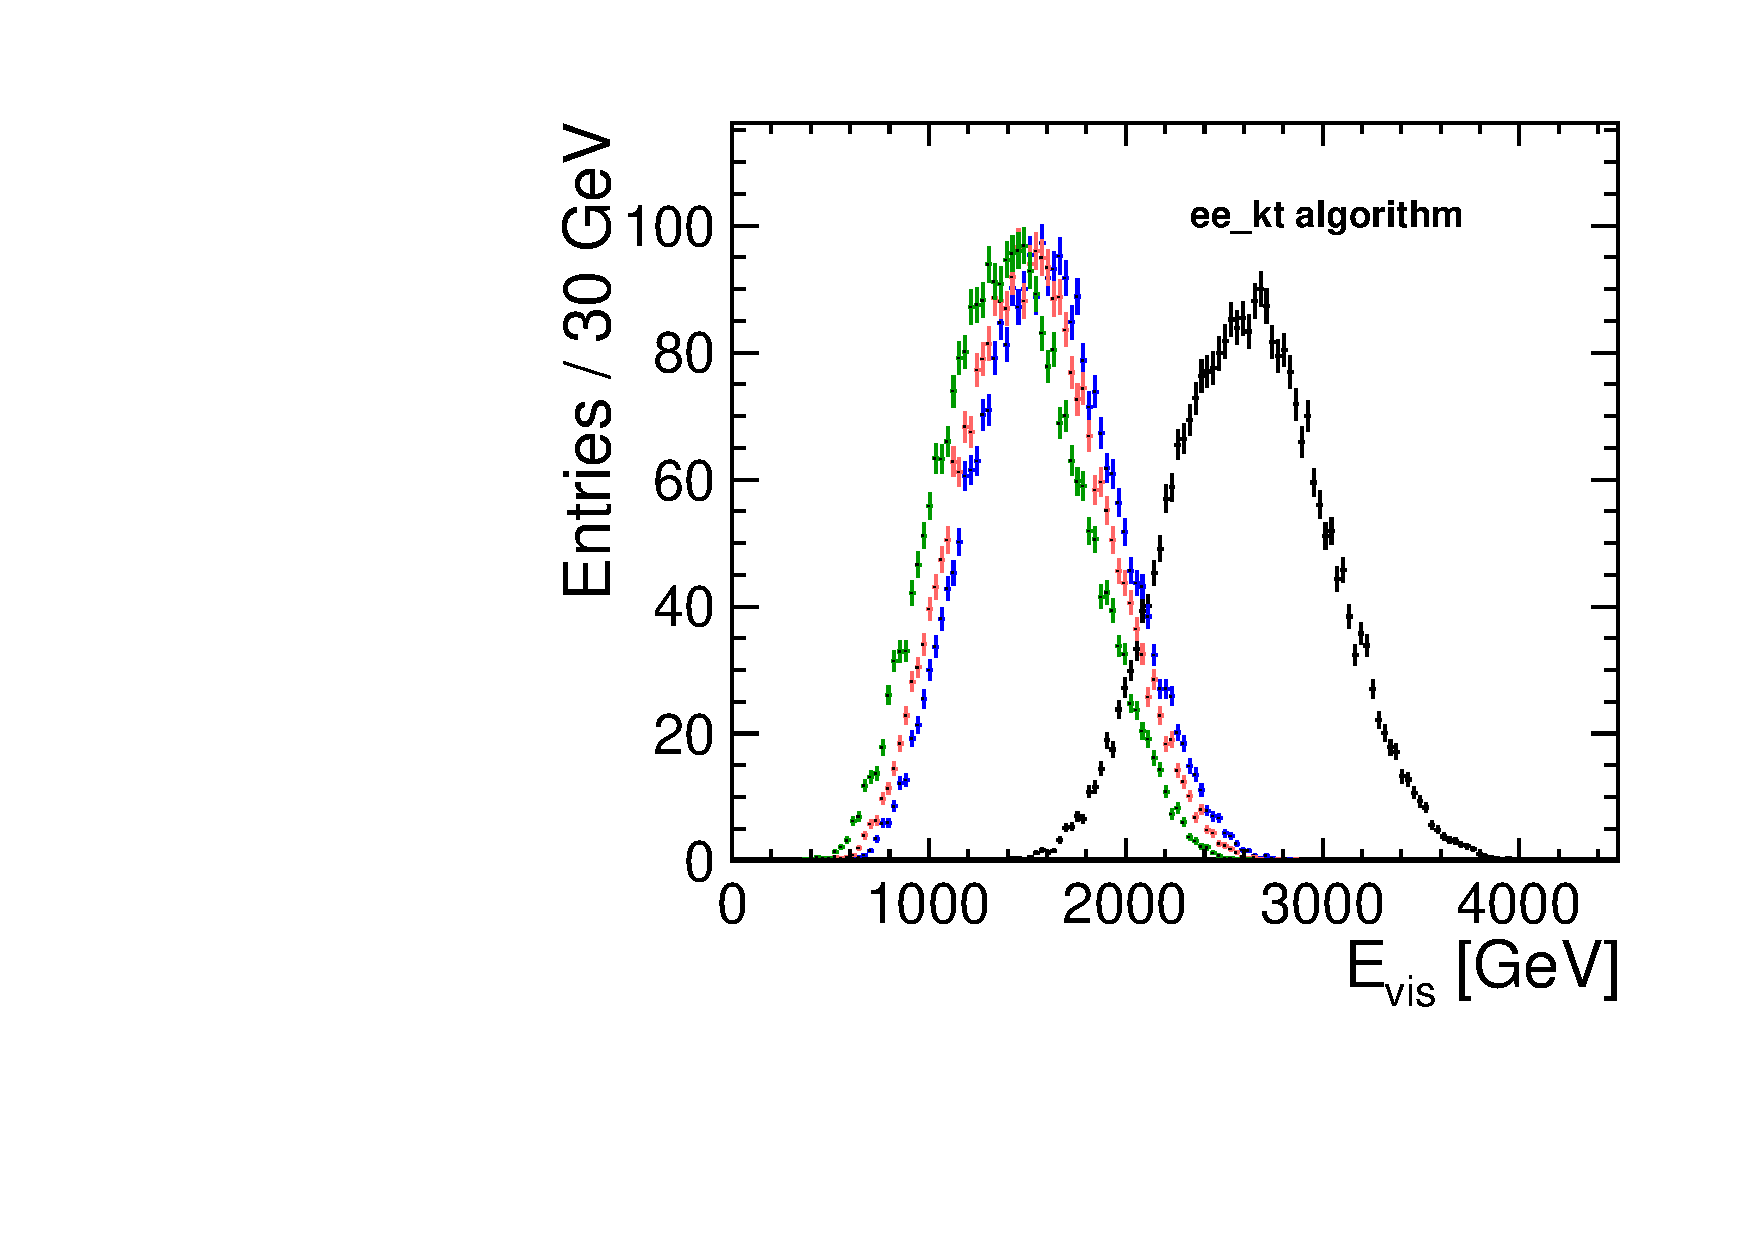
\includegraphics[width=6cm]{../SIDWorkshop/JetFinding_compare_E_vis__FJ_ee_kt_algorithm_ExclusiveNJets_2.pdf}\\
\column{6cm}
Hadron collider $k_{\textrm{T}}$:\\
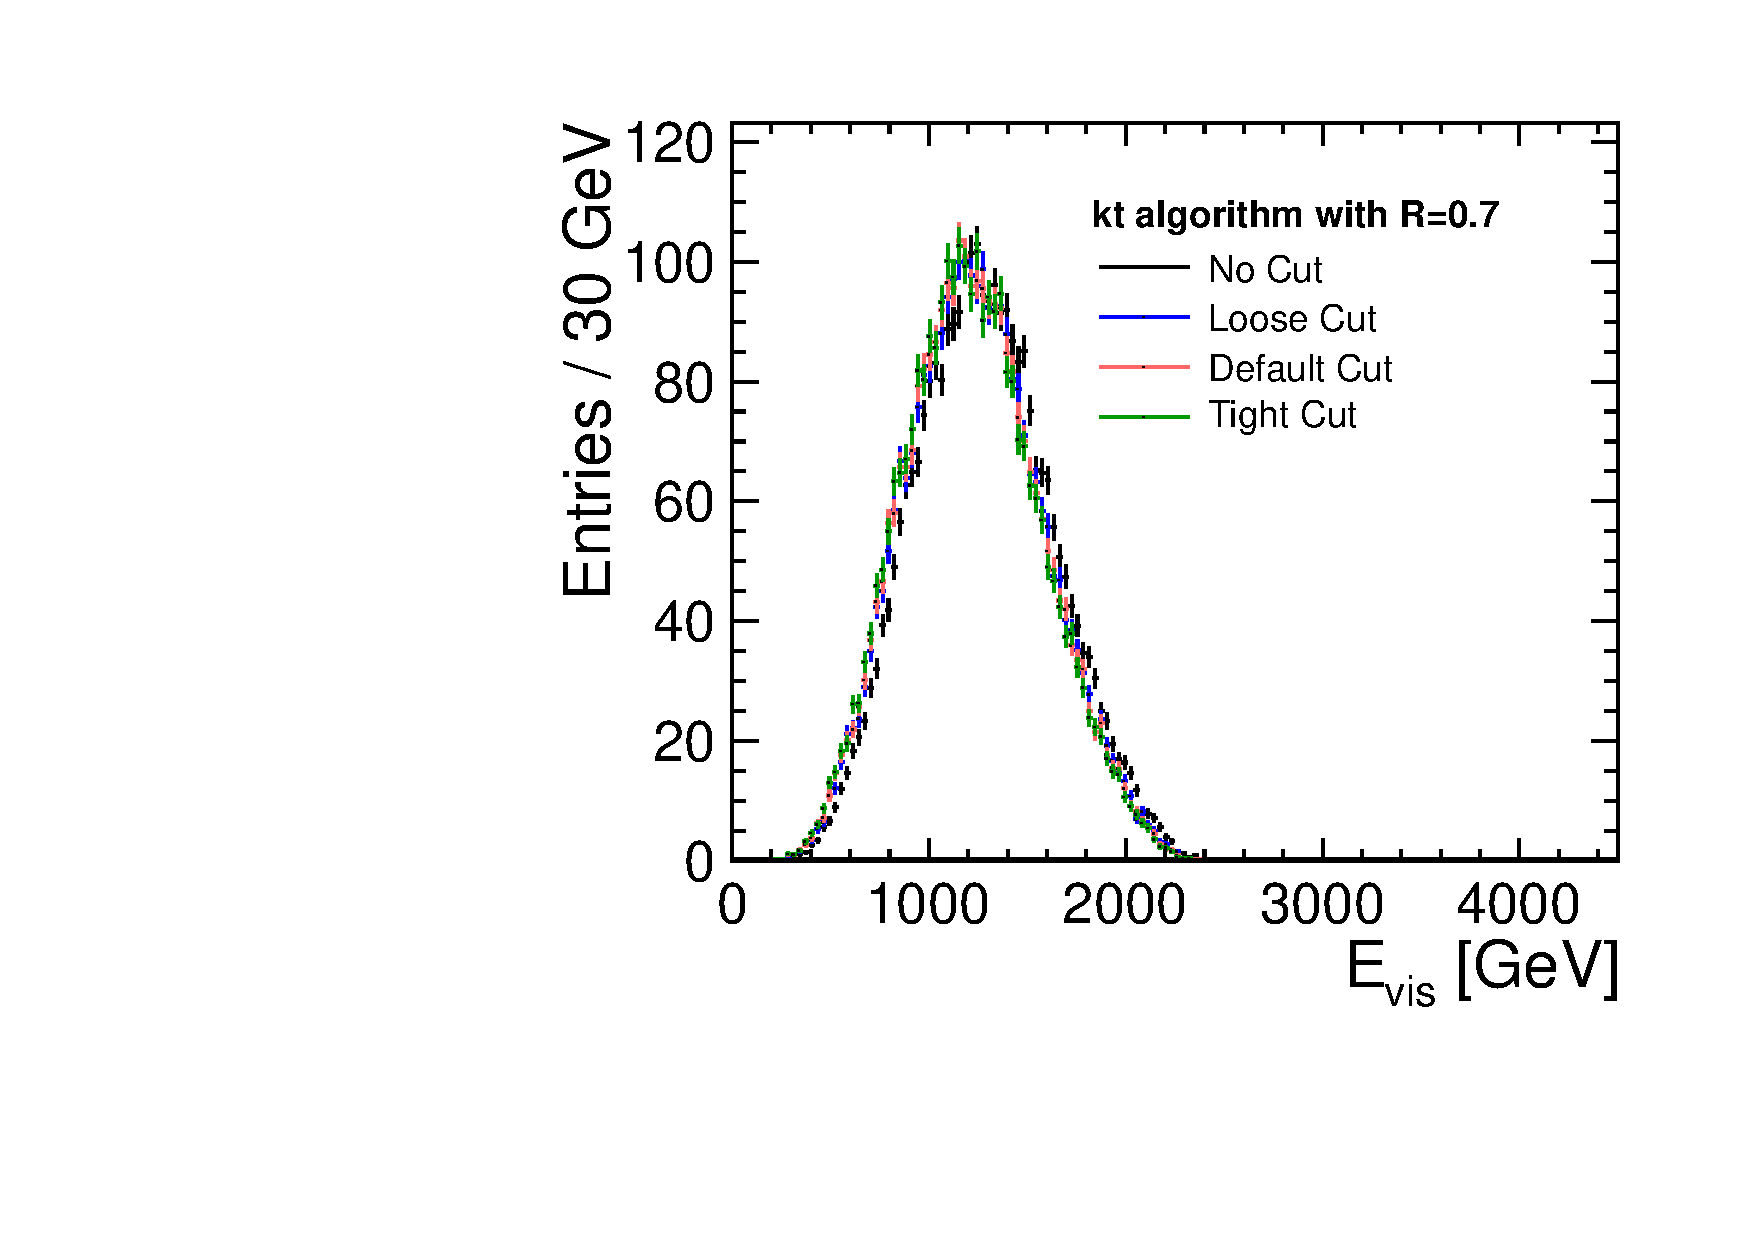
\includegraphics[width=6cm]{../SIDWorkshop/JetFinding_compare_E_vis__FJ_kt_algorithm_0_7_ExclusiveNJets_2.pdf}\\
\end{columns}
\begin{columns}
\column{6cm}
{\scriptsize
\begin{itemize}
  \item All particle clustered
  \item Timing cuts effective
\end{itemize}
}
\column{6cm}
{\scriptsize
\begin{itemize}
  \item Much of Bkg clustered with beam axis
  \item Timing cuts do less work
  \item Impact depends on event topology
\end{itemize}
}
\end{columns}
\end{frame}
\begin{frame}
\frametitle{Background suppression}
E.g. $\Pep\Pem\to\PH\PH\to\Ptop\APbottom\Pbottom\APtop$:
\begin{columns}[c]
\column{6cm}
\centering
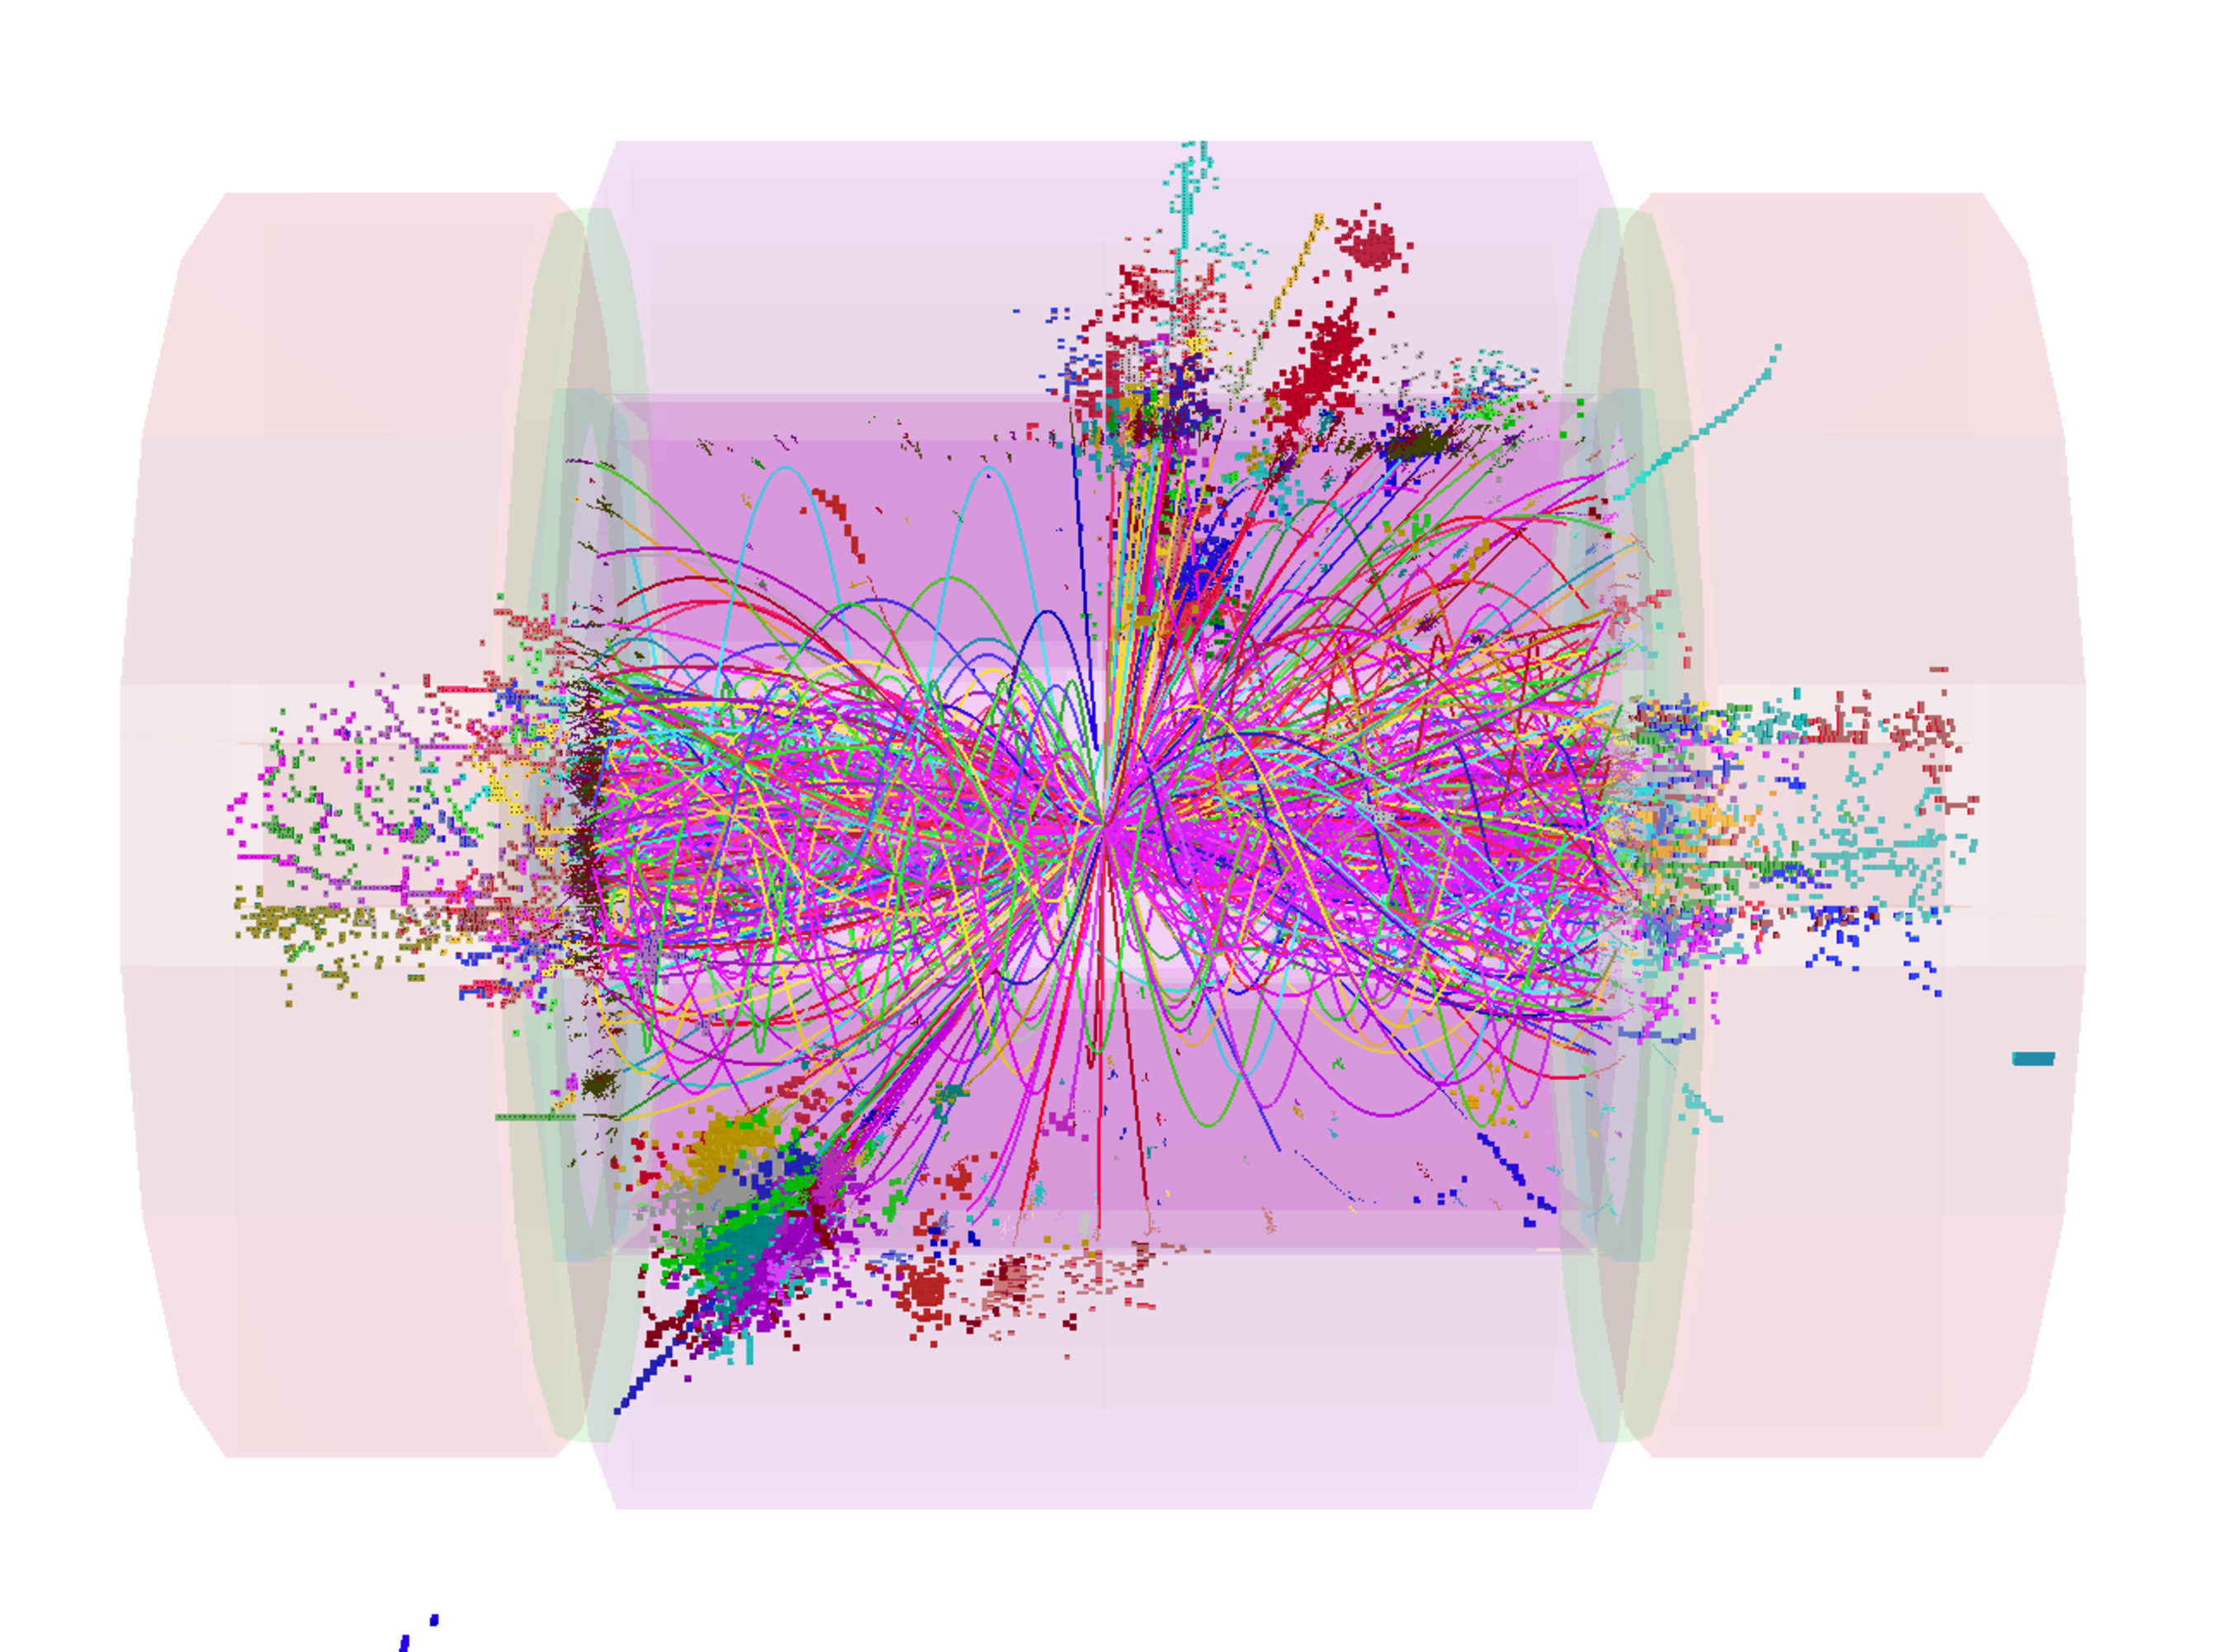
\includegraphics[width=6cm]{../SIDWorkshop/HH2.pdf}
\column{6cm}
\centering
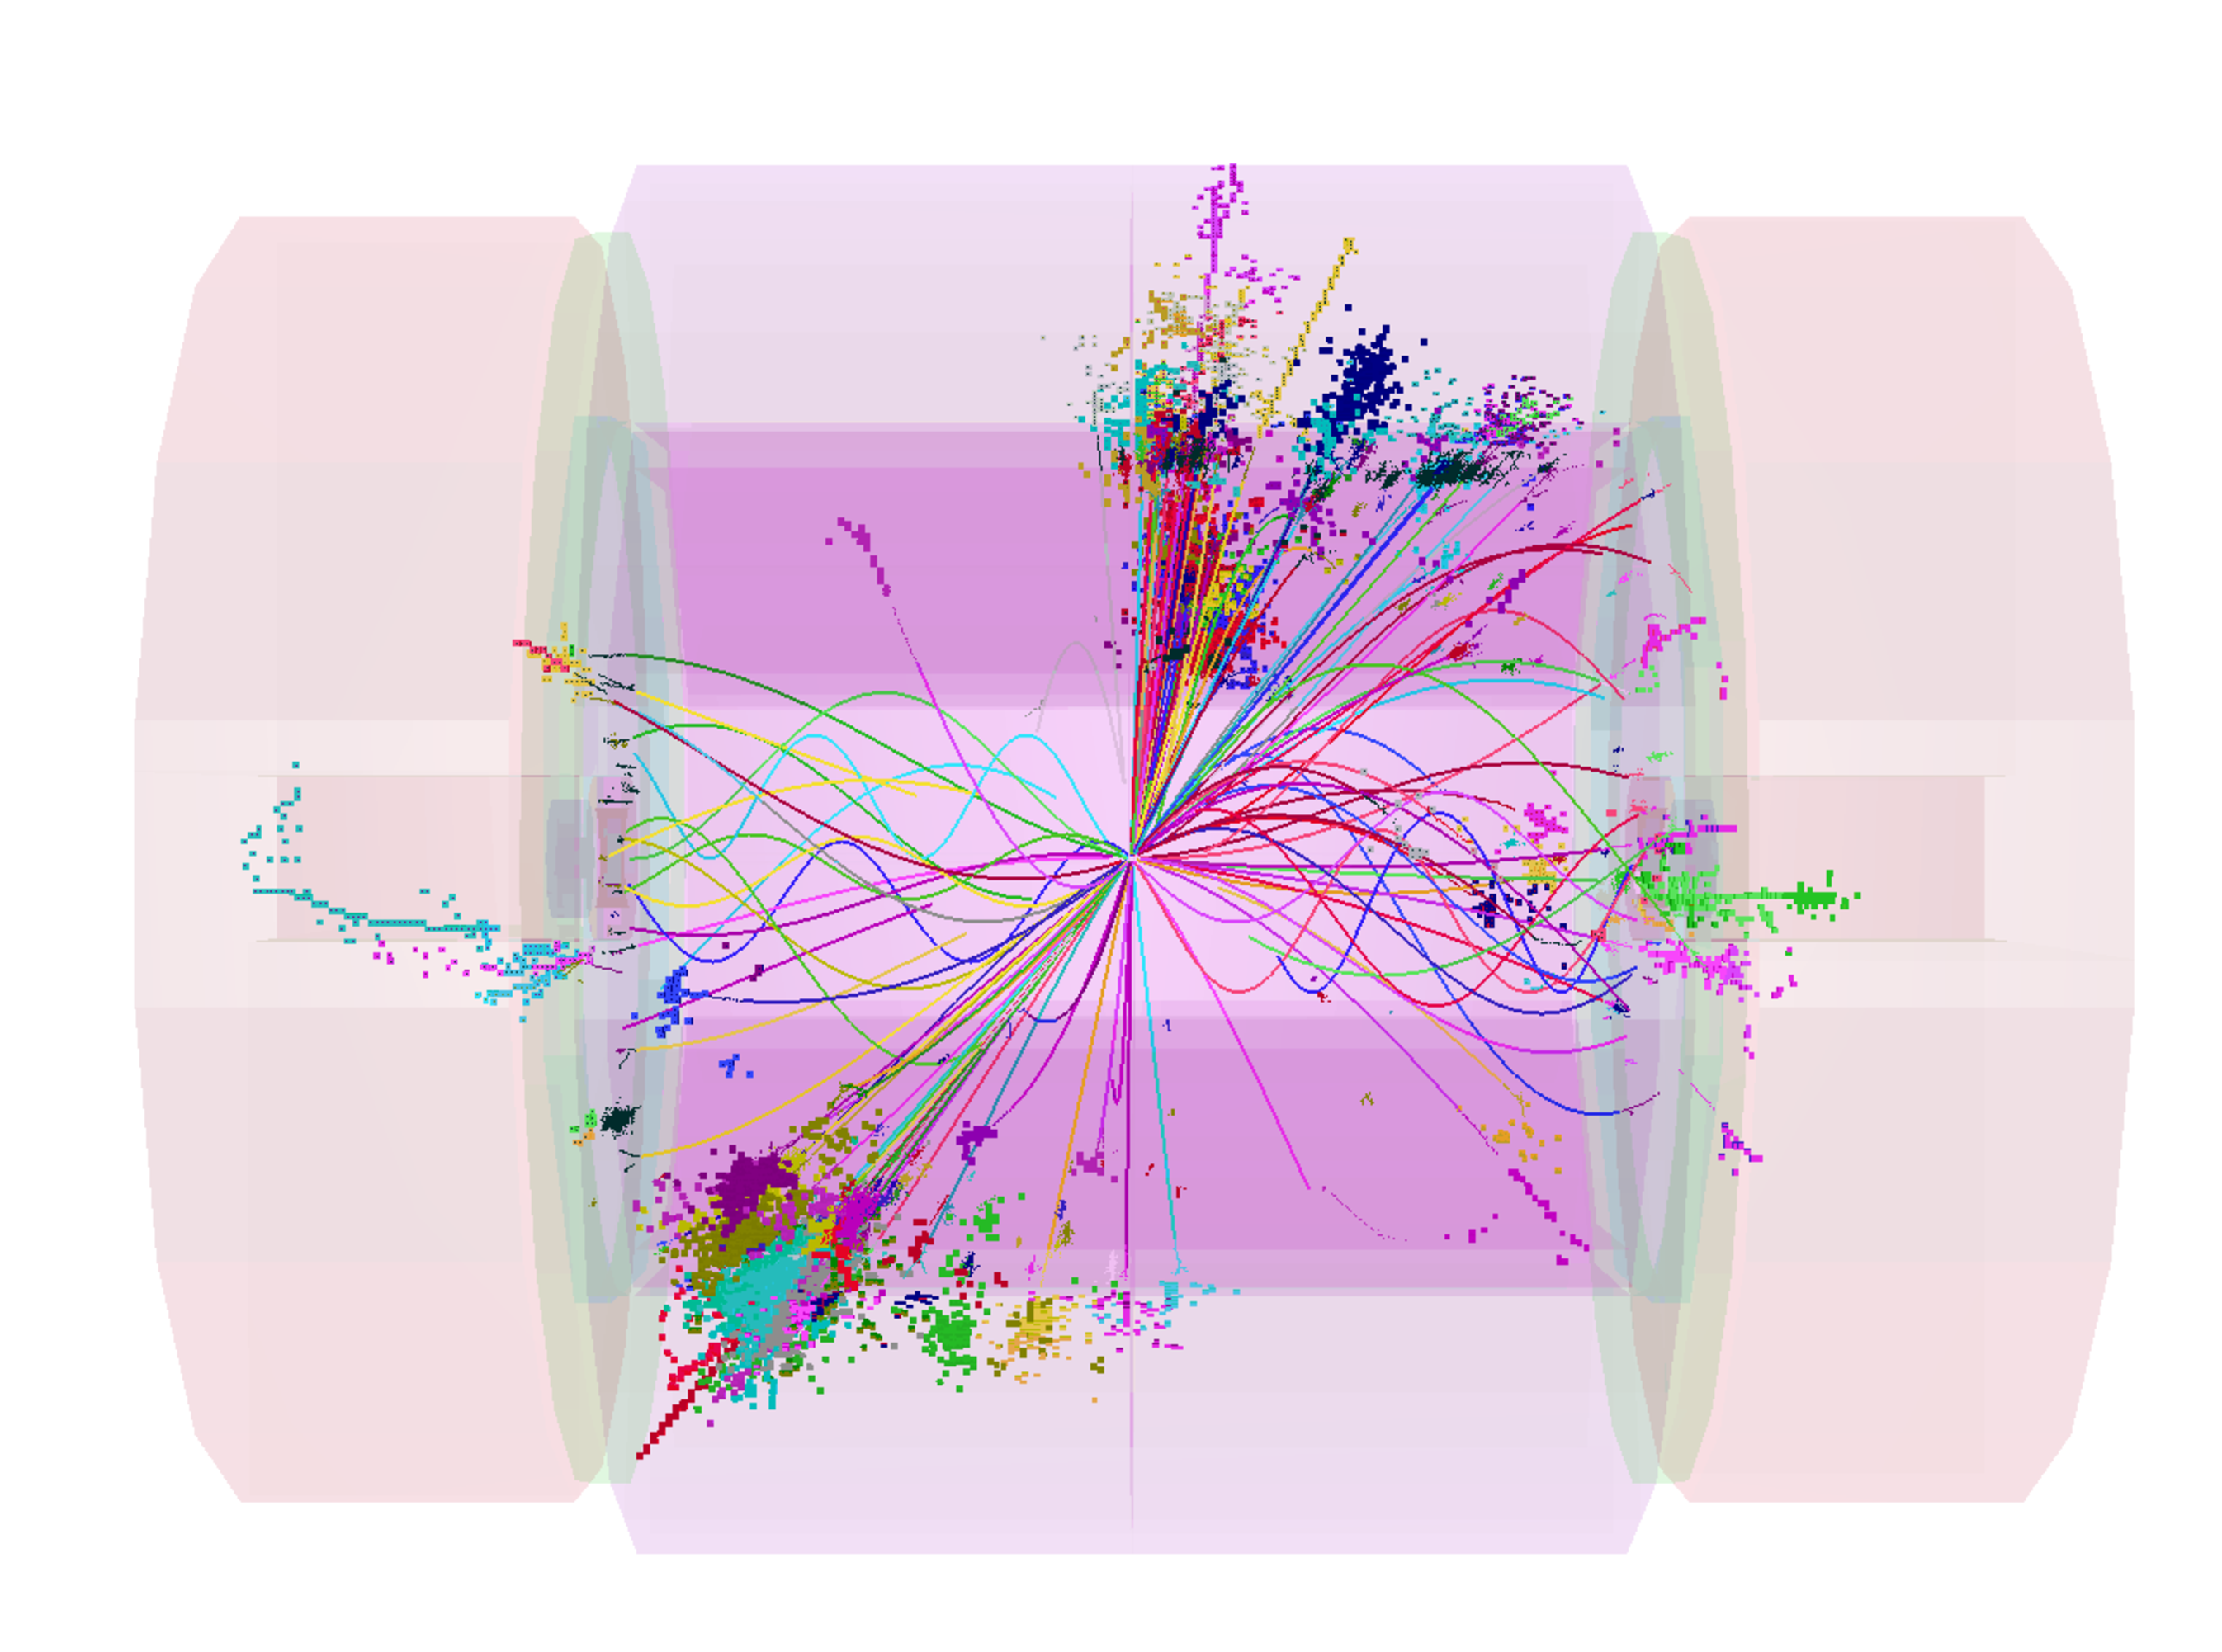
\includegraphics[width=6cm]{../SIDWorkshop/HH2tight.pdf}
\end{columns}
\begin{columns}[c]
\column{6cm}
\centering
No cuts:\\ \alert{$\sim1.2\textrm{TeV}$}\\
{\color{blue}{\scriptsize 10ns window}}
\column{6cm}
\centering
Tight timing cuts and jet finding:\\ \alert{$\sim100\textrm{GeV}$}
\end{columns}
~\\
\alert{Using timing cuts and jet finding removes most of the background}
\end{frame}

\section{Physics Results}
\begin{frame}
 \frametitle{Benchmark channels}
The benchmark channels used to assess detector performance:
\begin{itemize}
\item $\Pep\Pem \to \Ph \Pgne \Pagne, \Ph \to \mu^+\mu^-, \Ph \to
\Pbottom\APbottom$ (SID),
\item  $\Pep\Pem \to \PHp \PHm\to \Ptop\APbottom\APtop\Pbottom$(ILD),\\
$\Pep\Pem \to \PHz \PA\to\Pbottom\APbottom\Pbottom\APbottom$ (ILD),
\item $\Pep\Pem \to \PSq_R \PaSq_R\to\Pquark\APquark\PSgxz_1\PSgxz_1$ (ILD), 
\item $\Pep\Pem \to \PSl \PaSl \,(\ell = \Pe,\Pgm,\Pgne)$ (ILD), 
\item $\Pep\Pem \to \PSgxpm_1 \PSgxmp_1\to\PWp\PWm\PSgxz_1\PSgxz_1$ (SID),\\
$\Pep\Pem \to \PSgxz_2 \PSgxz_2\to \Ph\Ph\PSgxz_1\PSgxz_1$ (SID),
\item  $\Pep\Pem \to \Pqt \Paqt$ (500~GeV, ILD).
\end{itemize} 
\end{frame}
\begin{frame}
\frametitle{SM Higgs}
\end{frame}
\begin{frame}
\frametitle{SM Higgs}
\end{frame}
\begin{frame}
\frametitle{Squarks}
\end{frame}
\begin{frame}
\frametitle{Squarks}
\end{frame}
\begin{frame}
\frametitle{Sleptons}
\end{frame}
\begin{frame}
\frametitle{Sleptons}
\end{frame}
\begin{frame}
\frametitle{Gauginos}
\end{frame}
\begin{frame}
\frametitle{Gauginos}
\end{frame}
\begin{frame}
\frametitle{Heavy Higgs}
\end{frame}
\begin{frame}
\frametitle{Top physics at 500GeV: vertex detector}
\end{frame}
\begin{frame}
\frametitle{Top physics at 500 GeV: compare with ILC}
\end{frame}

\section{Conclusion}
\begin{frame}
\frametitle{Overview}
\begin{itemize}
  \item Introduced the CLIC machine
  \item Presented the CLIC detectors concept
  \item Shown that it's possible to deal with the machine induced background
  \item High precision physics possible
\end{itemize}
\end{frame}
\begin{frame}
\frametitle{Signatory list}
\textit{You are cordially invited to subscribe to the CDR Signatories List:\\
\begin{itemize}
\item If you have made contributions to the CLIC accelerator or the Linear
Colliders Physics and Detector studies, or intend to contribute in the future,
\end{itemize}
~\\
OR / AND\\
~\\
\begin{itemize}
  \item If you wish to express support to the physics case and the study of a
  multi-TeV Linear Collider based on the CLIC technology, and its detector
  concepts.
\end{itemize}
}
\url{https://indico.cern.ch/conferenceDisplay.py?confId=136364}
\end{frame}

\appendix
\begin{frame}
\frametitle{Backup slides}
\end{frame}
\section{Software}
\begin{frame}
\frametitle{Generation}
\end{frame}
\begin{frame}
\frametitle{Simulation}
\end{frame}
\begin{frame}
\frametitle{Handling background in the software}
\end{frame}
\begin{frame}
\frametitle{Reconstruction}
\end{frame}
\begin{frame}
\frametitle{Using the GRID: ILCDIRAC}
\end{frame}

\end{document}